% LARGE SCALE

\documentclass[preprint]{sigplanconf}

\usepackage{amsmath}
\usepackage{listings}
\usepackage{float}
\usepackage{graphicx}
\usepackage{adjustbox}
\usepackage{multirow}
\usepackage{color}

\newcommand{\ts}{\textsuperscript}

\newcommand{\cell}[2][c]{\begin{tabular}[#1]{@{}c@{}}#2\end{tabular}}
\renewcommand{\arraystretch}{1.2}

\floatstyle{ruled}
\newfloat{Listing}{tbp}{loa}

\begin{document}

\special{papersize=8.5in,11in}
\setlength{\pdfpageheight}{\paperheight}
\setlength{\pdfpagewidth}{\paperwidth}

\conferenceinfo{CONF 'yy}{Month d--d, 20yy, City, ST, Country} 
\copyrightyear{20yy} 
\copyrightdata{978-1-nnnn-nnnn-n/yy/mm} 
\doi{nnnnnnn.nnnnnnn}

% Uncomment one of the following two, if you are not going for the 
% traditional copyright transfer agreement.

%\exclusivelicense                % ACM gets exclusive license to publish, 
                                  % you retain copyright

%\permissiontopublish             % ACM gets nonexclusive license to publish
                                  % (paid open-access papers, 
                                  % short abstracts)

%\titlebanner{banner above paper title}        % These are ignored unless
%\preprintfooter{short description of paper}   % 'preprint' option specified.

\title{How Do Programmers Use Optional Typing? An Empirical Study}

\authorinfo{Carlos Souza}
           {Software Engineering Lab\\Federal University of Minas Gerais (UFMG)}
           {carlosgsouza@gmail.com}
\authorinfo{Eduardo Figueiredo}
           {Software Engineering Lab\\Federal University of Minas Gerais (UFMG)}
           {figureido@dcc.ufmg.br}

\maketitle

\begin{abstract}
The type paradigm is one of the most important things to be taken in consideration when choosing a programming language. 
This question has become increasingly important due to the recent popularization of dynamically typed languages such as Ruby and JavaScript. 
While, declaring types potentially improves the readability and maintainability of a program, it may require more work for the
programmer.
This paper presents a large scale empirical study with the goal of identifying programmers' points of views about these tradeoffs
An analysis of the source code of almost seven thousand projects written in Groovy, a programming language which features optional typing, shows in which situations programmers prefer typing or not their declarations. 
Results suggest that the need for maintainability, frequency of change and programmers background are important factors in this decision.
\end{abstract}

\category{D.2.3}{Software Engineering}{Cooding Tools and Techniques}

\terms
Experimentation, Language

\keywords
Type systems, static analysis, Groovy

\section{Introduction}
When choosing a programming language for a project, a developer considers several characteristics of that language.
One of the most important of these characteristics is its type system, which can be static or dynamic.
The type system determines when the type of a statement is defined \cite{types_and_programming_languages}. 
Statically typed languages, such as Java and C\#, require programmers to define the type of a declaration, which can then be used by the compiler to check for type errors. 
On the other hand, in dynamically typed languages, such as Ruby and JavaScript, the definition of the type of a statement only happens at run time.

Discussions about what is the best type system for a particular situation have become increasingly important in recent years due to rapid popularization of dynamically typed languages. 
According to the TIOBE Programming Community Index \cite{tiobe}, a well-known ranking that measures the popularity of programming languages, 27\% of the programming languages used in industry are dynamically typed. 
A decade ago, this number was only 17\%. 
Among the 10 languages on top of the ranking, four are dynamically typed: JavaScript, Perl, Python and PHP. 
None of these languages were among the top 10 rank until 1998.

Several factors may be considered when choosing between a dynamically or statically typed language. 
Since the type system of dynamically typed languages is simpler, they tend to allow programmers to code faster \cite{types_and_programming_languages} and adapt to frequently changing requirements more easily \cite{gradual_typing}.
Also, by removing the repetitive work of defining types, these languages allow programmers to focus on the problem to be solved rather than on the rules of the language \cite{dynamically_typed_languages}.

Statically typed languages also have their advantages. 
For instance, they allow compilers to find type errors statically \cite{should_your_specification_language_be_typed}. 
Typed declarations increase the maintainability of systems because they implicitly document the code, telling programmers about the nature of statements \cite{type_systems,mayer2012static}. 
Systems built with these languages tend to be more efficient since they do not need to perform type checking during execution \cite{bruce2002foundations,jit}. 
Finally, modern development environments, such as Eclipse and IDEA, are able to assist programmers with functionalities such as code completion based on the information provided by statically typed declarations \cite{bruch2009learning}.

Some languages try to combine characteristics from both static and dynamic type systems.
Groovy \cite{groovy} is one of these languages.
Although Groovy is mostly a dynamically typed language, it gives programmers the option to use type annotations as a means to document their code.
It is also possible to turn static type checking on so the compiler can find type errors before execution.
This allows developers to choose the most appropriate paradigm for each situation.

Understanding the point of view of programmers about the tradeoffs between type paradigms is an important matter.
Programmers can make an informed decision by knowing which languages provide the right benefits for their particular context.
Programming language developers can consider this information in their design so they can develop the most appropriate features for their target audience.
Finally, tools can be developed or improved to overcome any weaknesses of a given language. 

This paper presents a large scale empirical study about how programmers use optional typing in Groovy in order to understand which factors actually influence the decision of a developer for using types or not. 
This question was studied based on the analysis of a massive dataset with almost seven thousand Groovy projects.
Through a static analysis of these projects, it was possible to understand when developers use types and then extract what are the factors that influence this decision.

Results show that programmers consider types as a means to document their code.
This is even more evident on the definition of the interface of modules.
Conversely, when neither readability nor stability is a concern, programmers tend to type their declarations less often.
In addition to that, programmers seem to prefer the flexibility of untyped declarations in frequently changed code.
Finally, the experience of a programmer with other languages has a relevant influence on his or her choice for typing a declaration or not.

The remainder of this paper is organized as follows. 
Section \ref{groovy} introduces the main concepts of the Groovy programming language and Section \ref{settings} presents the study settings.
Section \ref{results} describes the results of the study, which are then discussed in Section \ref{discussion}.
Threats to the validity and related work are presented in Sections \ref{threats} and \ref{related} respectively.
Finally, Section \ref{conclusion} concludes this study and suggests future work.












%
%  THE GROOVY LANGUAGE
%

\section{The Groovy Language\label{groovy}}
Groovy is a dynamically typed programming language designed to run on the Java Virtual Machine.
Its adoption has grown remarkably over the last years.
According to the TIOBE Programming Index, Groovy is the 22\textsuperscript{nd} most popular language in the software industry \cite{tiobe}, ahead of languages like Prolog, Haskell and Scala. 
It builds upon the strengths of Java, but has additional features inspired by dynamic languages such as Python and Ruby.
Like Java, Groovy code is compiled to bytecode, allowing it to seamlessly integrate with existing Java classes and libraries. 
These factors have attracted a large number of Java programmers who want to use Groovy's dynamic functionality without having to learn a completely different language or change the execution platform of their systems. 

% Groovy was designed to be more expressive and concise than Java.
% Two implementations of a simple algorithm are shown below.
% Given a list of numbers, return a list containing only the even numbers of that list.
% Listing \ref{javaClass} shows the Java implementation while Listing \ref{groovyClass} shows the Groovy counterpart. 
% Because of its high level of expressiveness, Groovy is able to reduce much of the boilerplate required in Java.
% Listing \ref{groovyClass} shows that Groovy offers a native syntax for lists (lines 3, 6 and 14) and operator overloading (line 6). 
% Semicolons are optional, except when there are multiple statements in the same line. 
% When the keyword $return$ is omitted (line 10), the last expression evaluated with a method is returned. 
% Also, parentheses in method calls can often be omitted (line 16).
% In addition, Groovy implicitly imports frequently used classes, like those of the $java.util$ package, and methods, like $System.out.println$ (line % 16).

% \begin{Listing}[ht]
% \begin{lstlisting}[language=Java,tabsize=2,breaklines=true,numbers=left]
% import java.util.ArrayList;
% import java.util.List;
% 
% public class JavaFilter {
% 	List<Integer> evenNumbers(List<Integer> list) {
% 		List<Integer> result = new ArrayList<Integer>();
% 		for(int item : list) {
% 			if(item % 2 == 0) {
% 				result.add(item);
% 			}
% 		}
% 
% 		return result;
% 	}
% 
% 	public static void main(String[] args) {
% 		List<Integer> list = new ArrayList<Integer>();
% 		list.add(1);
% 		list.add(2);
% 		list.add(3);
% 		list.add(4);
% 
% 		List<Integer> result = new JavaFilter().evenNumbers(list);
% 		System.out.println(result);
% 	}
% }
% \end{lstlisting}
% \caption{A simple algorithm written in Java}
% \label{javaClass}
% \end{Listing}
% 
% \begin{Listing}[ht]
% \begin{lstlisting}[language=Java,tabsize=2,breaklines=true,numbers=left]
% class GroovyFilter {
% 	List<Integer> evenNumbers(List<Integer> list) {
% 		List<Integer> result = []
% 		for(int item : list) {
% 			if(item % 2 == 0) {
% 				result << item
% 			}
% 		}
% 
% 		result
% 	}
% 
% 	public static void main(String[] args) {
% 		List<Integer> list = [1, 2, 3, 4]
% 		List<Integer> result = new GroovyFilter().evenNumbers(list)
% 		println result
% 	}
% }
% \end{lstlisting}
% \caption{A simple algorithm written in Groovy}
% \label{groovyClass}
% \end{Listing}

% The design of Groovy was influenced by dynamic features of programming languages such as Ruby and Python.
% Listing \ref{dynamicInfuence} shows how these features can be used to rewrite the same algorithm presented % in Listing \ref{javaClass} in a single line of code. 
% First, notice that the code shown in Listing \ref{dynamicInfuence}  is a script, rather than a class file.
% It makes use of a closure to allow a programmer to define a filter logic.
% This closure is passed down to the \emph{findAll} method, which  apply this closure to every element of % the list to in order to decide if that element should be returned or not.
% Closures are one of the most important features of Groovy as compared to Java.
% They allow a functional programming style, which is both expressive and powerful.
% 
% \begin{Listing}[ht]
% \begin{lstlisting}[language=Java,tabsize=2,breaklines=true,numbers=left]
% println([1, 2, 3, 4].findAll {it % 2 == 0})
% \end{lstlisting}
% \caption{A class written in Groovy}
% \label{dynamicInfuence}
% \end{Listing}
% 
% Metaprogramming is another dynamic feature present in Groovy. 
% Listing \ref{metaprogramming} shows how to add a method to an existing class dynamically.
% By adding the method \emph{evenNumbers()} to the \emph{List} class, it is possible to achieve higher % expressiveness.
% This is specially useful when implementing Domain Specific Languages \cite{fowler10}.
% 
% \begin{Listing}[ht]
% \begin{lstlisting}[language=Java,tabsize=2,breaklines=true,numbers=left]
% List.metaClass.evenNumbers = {
% 	delegate.findAll {it % 2 == 0}
% }
% println([1, 2, 3, 4].evenNumbers())
% 
% \end{lstlisting}
% \caption{An example of metaprogramming in Groovy}
% \label{metaprogramming}
% \end{Listing}% 

When Groovy was first launched, in 2007, it was a purely dynamically typed language.
However, it allowed programmers to optionally type their declarations.
Examples of typed and untyped declarations combined in the same file are shown in Listing \ref{dynamicTyping}.
This kind of typing, however, should not be confused with static typing since the Groovy compiler does not use these type annotations to look for errors.
For example, the snippet of code shown in Listing \ref{typeError} compiles without any errors.
During runtime, the \emph{string} variable references an instance of the \emph{Integer} class.
However, an exception is thrown when we try to invoke the method \emph{toUpperCase} since the \emph{Integer} class does not have this method.

\begin{Listing}[ht]
\begin{lstlisting}[language=Java,tabsize=2,breaklines=true,numbers=left]
class DynamicTyping {
	private String typedField
	private untypedField

	DynamicTyping(typedParam) {}

	def untypedMethod(untypedParam, int typedParam) {
		def untypedVariable = 1.0
		return untypedVariable
	}

	int typedMethod()  {
		String typedVariable = ""
		return typedVariable
	}
}
\end{lstlisting}
\caption{Groovy is a dynamic language}
\label{dynamicTyping}
\end{Listing}

\begin{Listing}[ht]
\begin{lstlisting}[language=Java,tabsize=2,breaklines=true,numbers=left]
String string = new Integer(1)
string.toUpperCase()
\end{lstlisting}
\caption{A class written in Groovy}
\label{typeError}
\end{Listing}

Since version 2.0, Groovy allows programmers to explicitly activate static typing with the usage of the \emph{@TypeChecked} annotation.
This makes Groovy a gradually typed language \cite{gray05,gray08,gray11,siek07,takikawa12}.
In this mode, the Groovy compiler looks for type errors and fails if it finds any.
Listing \ref{staticTyping} shows an example of static typing in Groovy.
Trying to compile the class \emph{TypeCheckedGroovyClass} produces an error since the method \emph{sum} is supposed to receive two parameters of the type \emph{int}, but it is actually called with two parameters of the type \emph{String}.

\begin{Listing}[ht]
\begin{lstlisting}[language=Java,tabsize=2,breaklines=true,numbers=left]
@TypeChecked
class TypeCheckedGroovyClass {
	
	static int sum(int a, int b) {
		a + b
	}

	public static void main(String[] args) {
		println sum("1", "2")
	}
}
\end{lstlisting}
\caption{A class written in Groovy}
\label{staticTyping}
\end{Listing}

The \emph{@TypeChecked} annotation is reasonably recent and most Groovy programmers still do not use it. 
Typing annotations on the other hand are very popular.
Although they do not provide static type checking, they are capable of documenting the code and aiding in the integration with development tools.
In the remainder of this text, we refer to declarations with type annotations as "typed", while the word "untyped" is used for declarations with no type annotations.







%
% STUDY SETTINGS
%

\section{Setudy Settings\label{settings}}
% Be more objective in the begining. DRY
The study presented in this paper consists in the static analysis of the source code of a corpus of 6638 Groovy projects with the goal of finding the factors that have an actual influence over the decision of a developer to type their declarations or not. 
In this section we present the research questions we want to answer, the data collection and analysis procedures as well as the characterization of the studied dataset.

\subsection{Research Questoins\label{questions}}
Static and dynamic type system have known advantages and disadvantages.
We propose some research questions below in order to find which ones are actually considered by programmers in their code.

\begin{itemize}
	\item \textbf{Question Q1: Do programmers use types to implicitly document their code?} By typing their declarations, developers are telling their colleagues (or themselves) about the nature of those declarations. This increases the readability and, hence, the maintainability of their code. If we are able to observe a higher usage of types in declarations that usually require more documentation, then we can assume that these developers indeed consider types as a means to document their code.
	\item \textbf{Question Q2: Are untyped declarations preferred when neither readability nor stability is a concern?} Besides readability, typing also contributes to stability. It reduces the risk of unexpected effects of modifications increasing the maintainability of the software system \cite{Iso2004}. Our hypothesis is that, where these are not important factors, typing becomes less necessary and developers prefer the simplicity and flexibility offered by dynamic typing. 
	\item \textbf{Question Q3: In frequently changed code, do developers prefer typed or untyped declarations?} It makes sense to assume that developers try to increase the maintainability of frequently changed files. One way to achieve that is improving the readability of such code with the use of types. On the other hand, the flexibility of untyped declarations is capable of increasing the changeability of those files. We want to understand which one of these strategies is actually preferred by developers in the end.
	\item \textbf{Question Q4: Does the previous experience of programmers with other languages influence their choice for typing their code?} We believe that programmers familiar with a statically typed language keep using types since they are used to it. 
\end{itemize}

\subsection{Data Collection Procedure\label{dataCollection}}
The projects used in this study were obtained from GitHub, a popular source control service based on Git.
For each project, it was necessary to retrieve its source code, metadata, commit history, and the metadata of all of its developers.
GitHub does not offer a listing of all hosted projects, but it offers two search mechanisms, a REST API and a web based search page.
Unfortunately the GitHub API is too limited for our requirements.
It imposes a limit of one thousand results and does not allow filtering projects by their programming language.

In order to retrieve an extensive dataset, it was necessary to write a bot to simulate human interactions with the GitHub webpage and search for projects. 
Some special care was necessary to make this work. 
For instance, because the number of results is limited to 1 thousand projects, we had to segment the queries.
Multiple requests were made, and each one asking for the name of all projects created on a given month.
Results were then combined into a single list.
Another problem faced was that GitHub denies excessive requests from the same client.
By adding a 10 seconds delay between requests, it was possible to overcome this limitation.

With the name of all projects in hands, it was then possible to use the GitHub REST API to query their metadata.
That metadata also contains the identifiers of the developers and of the commits of that project.
Using those identifiers we once again used GitHub REST API and obtained the background of all developers and the file changes of all projects.


%DATASET
\subsection{Dataset\label{dataset}}

% count scripts, main classes and test classes

Our dataset consists of 6638 projects with almost 9.8 million lines of code.
Table \ref{tab:dataset_characterization} shows descriptive statistics for the size, age and number of commits of these projects.
There are more than 1.5 million declarations of all types and visibilities in our dataset.
More details about these declarations are shown in Table \ref{tab:number_of_declarations}.

\begin{table}[h!]

\centering{}%
\renewcommand{\arraystretch}{1.2}

\begin{tabular}{|c|c|c|c|c|c|}
\hline
{}		& Mean	& Median	& Std. Dev.	& Max	& Total		\\
\hline
\hline
Size (LoC)	& 1471 	& 529  & 4545  & 149933	& 9770783	\\ \hline
Commits   	& 31  	& 5    & 175   & 6545		& 203375	\\ \hline
Age (Days)  & 361  	& 280  & 333   & 1717		& 2395441	\\ \hline
\end{tabular}
\caption{Dataset characterization}
\label{tab:dataset_characterization}
\end{table}

\begin{table}[h!]

\centering{}%
\renewcommand{\arraystretch}{1.2}

\begin{tabular}{|c|c|c|c|c|c|}
\hline
{}		& Mean	& Median	& \cell{Std.\\Dev.}	& Max	& Total		\\
\hline
\hline
\cell{Field}                      	&   54    &  19  &    163  &    5268 & 366148   \\ \hline                  
\cell{Constructor\\Parameter}     	&    3    &   0  &     16  &     933 &  18956   \\ \hline                  
\cell{Method\\Parameter}          	&   30    &   6  &    110  &    3554 & 202617   \\ \hline                  
\cell{Method\\Return}             	&   53    &  15  &    165  &    4893 & 357997   \\ \hline                  
\cell{Local\\Variable}            	&   88    &  21  &    361  &   16427 & 602645   \\ \hline                  
\hline																			
Public                    			&   74    &  20  &    239  &    7942 & 507296   \\ \hline                  
Protected                 			&    6    &   0  &     32  &    1394 &  42646   \\ \hline                  
Private                   			&   58    &  21  &    178  &    5268 & 395776   \\ \hline                  
\hline																			
All                       			&  227    &  71  &    744  &   29862 &1548363   \\ \hline                  
\end{tabular}
\caption{Number of Declarations}
\label{tab:number_of_declarations}
\end{table}


More than 4 thousand developers were involved in the projects in our dataset.
While 96\% of the projects were developed by small groups of 3 people or less, there were projects with up to 58 people.
These developers have different backgrounds.
Figure \ref{fig:other_languages} shows what are the most popular languages used by these developers in other GitHub projects. 
Java is the most popular among them.
More than 50\% of the developers of projects in our dataset also have Java projects hosted on GitHub.

% Figure \ref{fig:typeSystem_background} shows what is the type system of the languages the developers in our dataset have experience with.
% Most of them have experience with both statically and dynamically typed languages.
% There are two small groups however that have experience with only one type system outside Groovy.
 
% \begin{table}[ht]
% \caption{Distribution of the Number of Developers in a Project}
% \centering{}%
% \begin{tabular}{|c|c|c|}
% \hline 
% Number of Developers & Fraction of Projects\tabularnewline
% \hline 
% \hline 
% 1 & 84\%\tabularnewline
% \hline 
% 2 & 9\%\tabularnewline
% \hline 
% 3 & 3\%\tabularnewline
% \hline 
% 4 or more & 4\%\tabularnewline
% \hline 
% \end{tabular}
% \label{tab:number_of_developers}
% \end{table}

\begin{figure}[h]
\centering 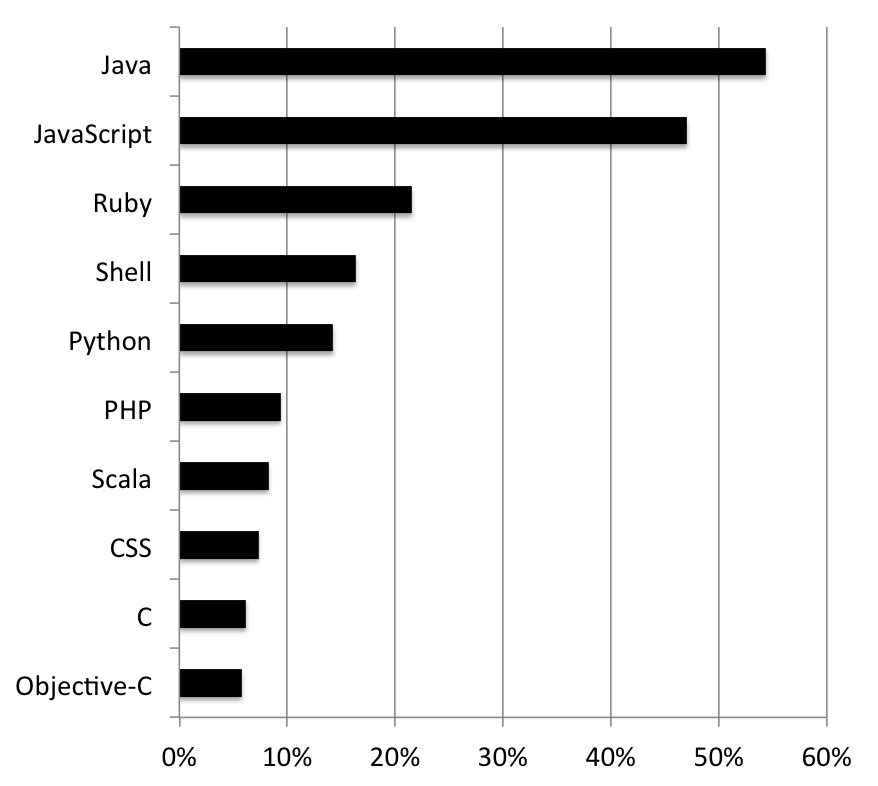
\includegraphics[width=0.45\textwidth]{other_languages}
\caption{Usage of other languages by Groovy developers on GitHub}
\label{fig:other_languages} 
\end{figure}

% \begin{figure}[ht]
% \centering 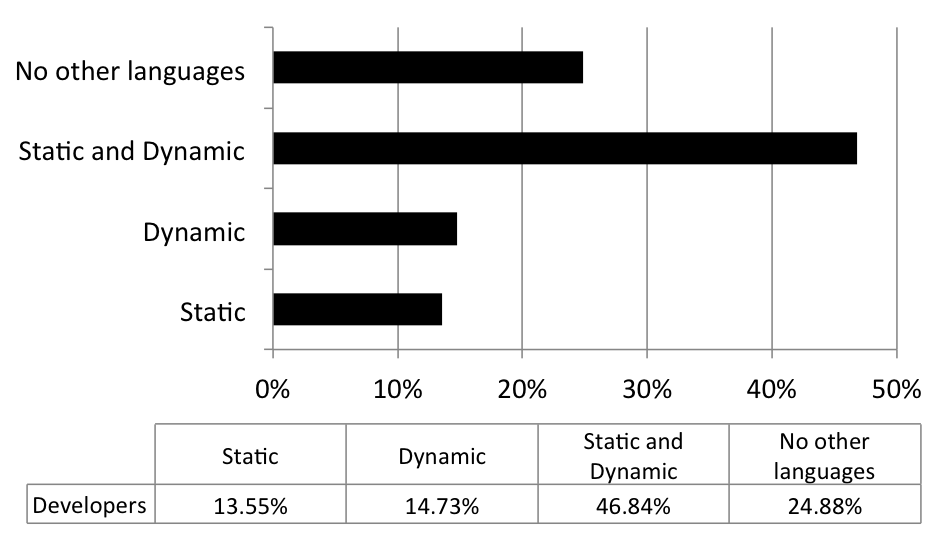
\includegraphics[width=0.45\textwidth]{typeSystem_background}
% \caption{Type System of other languages used by programmers}
% \label{fig:typeSystem_background} 
% \end{figure}



%ANALYSIS
\subsection{Analysis\label{analyzer}}
In order to understand where programmers use types, we developed a static code analyzer based on the Groovy metaprogramming library.
It is capable of retrieving the declaration information of parameters and returns of methods, parameters of constructors, fields and local variables.
In addition, it can tell if a declaration is part of a test class or a script and what is its visibility.

A relevant decision we made was not to compile projects, which would require all dependencies to be resolved.
This is not feasible given the size of our dataset.
Instead, we generated the AST for each file using the $CONVERSION$ phase of the Groovy compiler.
At this phase, the compiler has not tried to resolve any dependencies yet, but it is capable of generating an AST with enough information to determine if a a declaration is typed or not.
This makes it possible to analyze each Groovy file separately without having to compile the whole project.

The downside of the approach described above is that we can not analyze Groovy code in conjunction with its dependencies. 
For example, it is impossible to determine whether programmers tend to type code that interacts with other typed modules since we have not resolved any dependencies to these modules.
However, our choice was fundamental in order to execute a study with such an extensive dataset.
Nevertheless, as shown in the next section, we were still able to obtain detailed and relevant results.











%
% RESULTS
%
\section{Results\label{results}}
% TODO
% Be more objective
% Describe analysis strategy here
% Subsection \ref{res-type-visibility} shows the type usage in different sorts of declarations and visibilities.
% Subsection \ref{res-test-scripts} shows results depending on the type of the file where a declaration was made, a script, a class or a test class.
% The effects of the programmers' background and the project size are described in the Subsection \ref{res-background} and \ref{res-size}.
% Finally Subsection \ref{res-changes} presents results according to the number of changes of files.
% These results will be further discussed in Section \ref{discussion} in order to answer the research questions proposed in Section \ref{questions}.

\subsection{Overall Result\label{res-overall}}
Figure \ref{fig:all_histogram_all} gives an overview of the usage of types in all projects in our dataset.
It shows the mean, standard deviation and the quartiles of the relative use of types in a project. 
This value can vary from 0, in case a project does not declare any types, to 1, in case all declarations of a project are typed. 
% TODO: show, show, show...
This result is shown in more details on a histogram in , which shows the distribution of the values of relative use of types across all 6638 projects.
% TODO: Discuss results a little more?


\begin{figure}[h]
\centering 
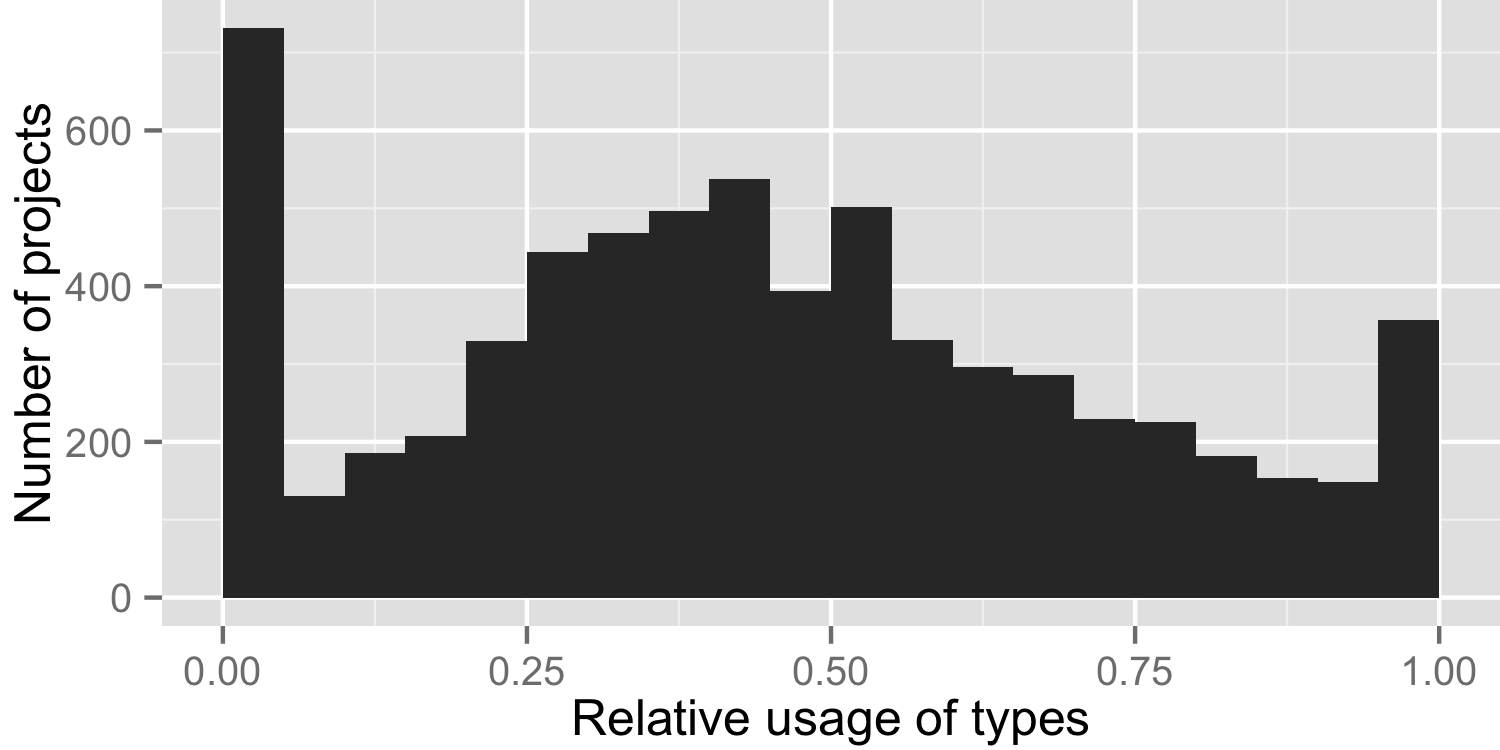
\includegraphics[width=0.45\textwidth]{../analysis/result/all/histograms/5_all_types.png} 

\vspace{0.3cm}
\small
\begin{tabular}{|c|c|c|cccc|}
\hline
{}		&  {}		&  {}			&  \multicolumn{4}{c|}{Quartiles}				\\
n		& mean	& std. dev.	& 1\ts{st}	& 2\ts{nd}	& 3\ts{rd}	& 4\ts{th}		\\
\hline
\hline
6638 	& 0.45	& 0.28		& 0.25	& 0.42		& 0.64	& 1.00		\\
\hline
\end{tabular}


\caption{Usage of types in all declarations of all projects}
\label{fig:all_histogram_all} 
\end{figure}



% TYPE
\subsection{Declaration Type\label{sub:res_all_type}}
The relative use of types per type of declaration is shown in Figure \ref{fig:all_boxplot_type} along with the corresponding descriptive statistics.
Each box plot in this graph describes relative use of types in five sorts of declarations: fields, parameters of constructors, parameters and returns of methods and local variables.
It considers all declarations of all projects.
Note that the value of n is different for each element in the table since not all projects have all types of declarations. 

\begin{figure}[h]
\centering 
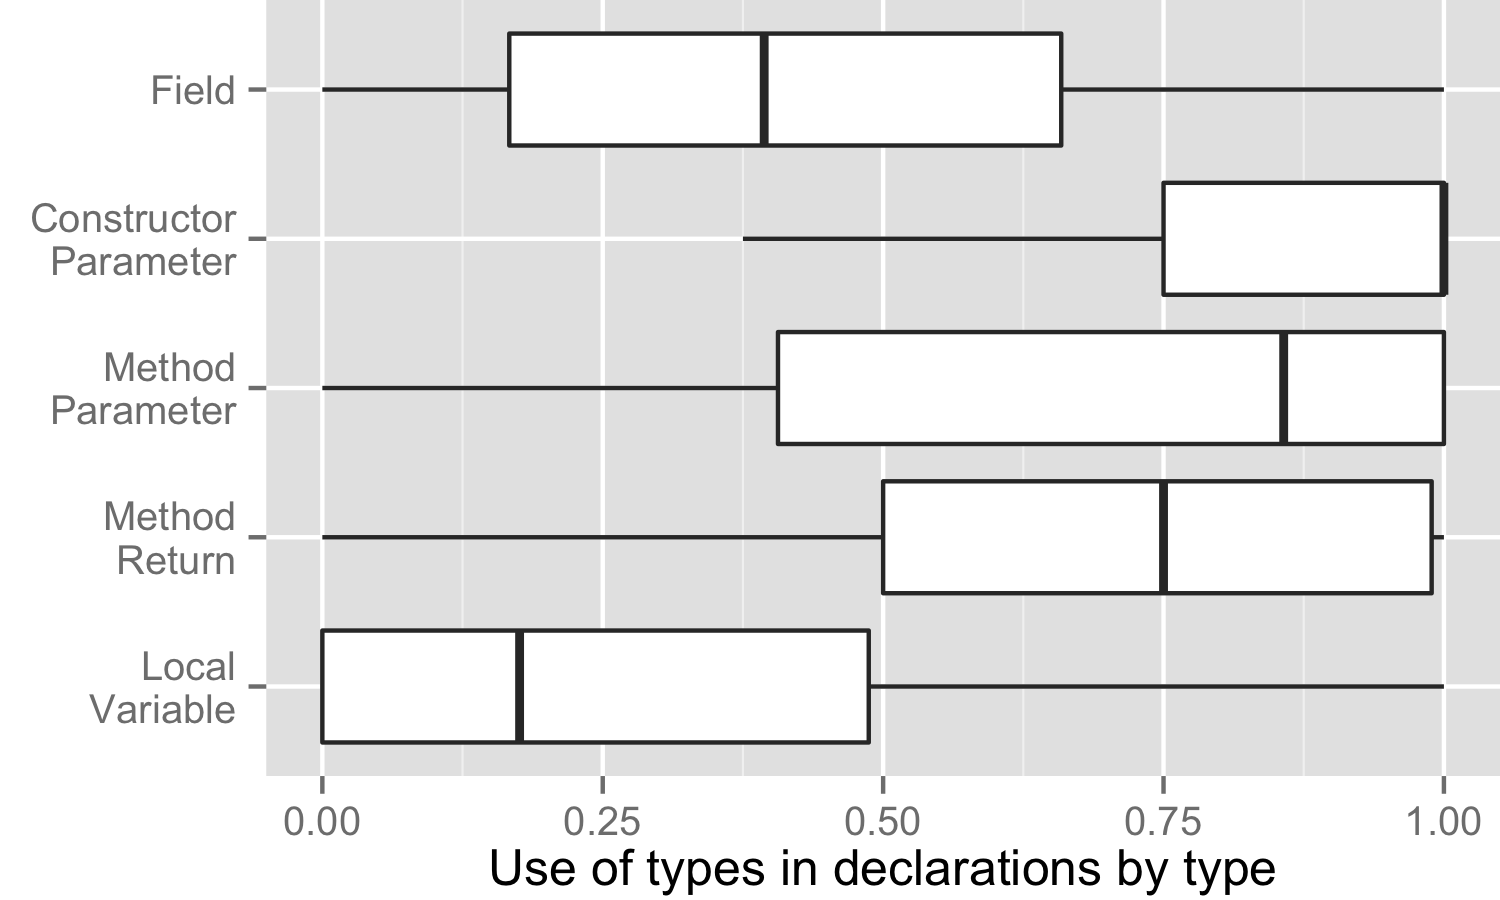
\includegraphics[width=0.45\textwidth]{../analysis/result/all/boxplots/6_declarations_by_type.png} 
\label{fig:all_boxplot_type} 

\vspace{0.3cm}

\renewcommand{\arraystretch}{1.2}
\small
\begin{tabular}{|c|c|c|c|c|}
\hline
Declaration Type		& n		& mean	& median		& std. dev.	\\
\hline
\hline
Field					& 6000	& 0.43	& 0.39		& 0.33		\\ \hline
Constructor Parameter	& 1670	& 0.80	& 1.00		& 0.35		\\ \hline
Method Parameter		& 4867	& 0.67	& 0.86		& 0.36		\\ \hline
Method Return			& 5881	& 0.68	& 0.75		& 0.31		\\ \hline
Local Variable			& 5845	& 0.29	& 0.18		& 0.32		\\ \hline
\end{tabular}

\caption{Usage of types in all declarations by type of declaration}

\end{figure}

The results presented in Figure \ref{fig:all_boxplot_type} suggest that programmers use types differently depending on the type of declaration.
Local variables for example are typed less often.
Half of the projects have 18\% or less of their local variables typed.
Conversely, methods and constructors are typed most of the cases.
Note that the median for constructor parameters is equal to 1.00, which means that, at least, half of the projects with constructor parameters type all declarations of this kind.

In order to check whether there is a significant difference in the use of types in two kinds of declaration, a significance test should be applied. 
We start by defining a hypothesis below. A significance test can be applied to reject or accept the null hypothesis, H0, for any two declaration types. 

\begin{description}
\item[H0] The data for two declaration types are drawn from the same population, i.e., there is no difference in how programmers type different types of declarations
\item[H1] Programmers type their declarations differently depending on the type of the declaration
\end{description}

We can not assume that the data presented in Figure \ref{fig:all_boxplot_type} follows any particular distribution.
In fact, an analysis of the data for declarations of local variables, methods and constructors shows that these samples are heavily skewed and thus do not follow a Normal distribution.
Because of this, we are required to use a non-parametric test to analyze this data.

An appropriate test for our scenario is the paired Mann-Whitney U test.
This test computes a p value indicating whether two samples are significantly different form each other.
The smaller the value of p, the "more significant" is the difference and, consequently, the stronger the rejection of the null hypothesis.
Typically values of 0.05 and 0.01 are used to determine if the null hypothesis can be rejected or not.
In addition to p, the Mann-Whitney U test also reports a confidence interval describing the difference of the medians of two populations.
This confidence interval can be used to measure how different are two samples.

% Use a super small significance level
% Labovitz, Sanford. "Criteria for selecting a significance level: A note on the sacredness of. 05." The American Sociologist 3.3 (1968): 220-222.

\begin{table}[ht]

\centering{}%
\renewcommand{\arraystretch}{1.2}

\begin{tabular}{|c|c|c|c|}
\hline 
								& {}					& p  	      & conf. interval\\
\hline
\hline
\multirow{4}{*}{Field}			& Constructor Parameter	& 0.0000 & (-0.50,-0.44)\\
								& Method Parameter		& 0.0000 & (-0.32,-0.27)\\
								& Method Return			& 0.0000 & (-0.30,-0.26)\\
								& Local Variable 		& 0.0000 & ( 0.13, 0.17)\\
\hline
{}								& Field					& 0.0000 & (0.44, 0.50)	\\
Constructor						& Method Parameter		& 0.0000 & (0.06, 0.09)	\\
Parameter						& Method Return			& 0.0000 & (0.08, 0.13)	\\
{}								& Local Variable		& 0.0000 & (0.62, 0.67)	\\
\hline
{}								& Field					& 0.0000 & ( 0.27,  0.32)	\\
Method							& Constructor Parameter	& 0.0000 & (-0.09, -0.06)	\\
Parameter						& Method Return			& 0.0054 & ( 0.00,  0.00)	\\
{}								& Local Variable		& 0.0000 & ( 0.44,  0.50)	\\
\hline
{}								& Field					& 0.0000 & ( 0.26,  0.30)	\\
Method							& Constructor Parameter	& 0.0000 & (-0.13, -0.08)	\\
Return							& Method Parameter		& 0.0054 & ( 0.00,  0.00)	\\
{}								& Local Variable		& 0.0000 & ( 0.44,  0.47)	\\
\hline
{}								& Field					& 0.0000 & (-0.17, -0.44) \\
Local							& Constructor Parameter	& 0.0000 & (-0.67, -0.27) \\
Variable						& Method Parame			& 0.0000 & (-0.50, -0.26) \\
{}								& Method Return			& 0.0000 & (-0.47,  0.17) \\
\hline  
\end{tabular}
\label{tab:all_utest_type}
\caption{Mann-Whitney U Test results for the comparison between the usage of types by type of declaration}
\end{table}

Table \ref{tab:all_utest_type} shows the result of the Mann-Whitney U test for the data displayed in Figure \ref{fig:all_boxplot_type}.
Confidence intervals are calculated with a confidence of 95\%.
All p values are close to 0, allowing us to strongly reject the null hypothesis for all test executions.
Note however that the confidence interval for the comparison between method parameters is negligible.


% VISIBILITY
\subsection{Declaration Visibility\label{sub:res_all_visibility}}
Figure \ref{fig:all_boxplot_visibility_all} shows how programmers use types depending on the visibility of a declarations.
Results consider all sorts of declaration, except for local variables which do not have visibility. 
We follow the same approach from previous section and apply the Mann-Whitney U test to determine whether there is a significant difference between declarations of different visibilities.
Results for the tests executions are displayed in Table \ref{tab:all_utest_visibility}.
They show that the p value for all tests is equal to 0, which points out that all declarations visibilities are different from each other.

\begin{figure}[h]
\centering 
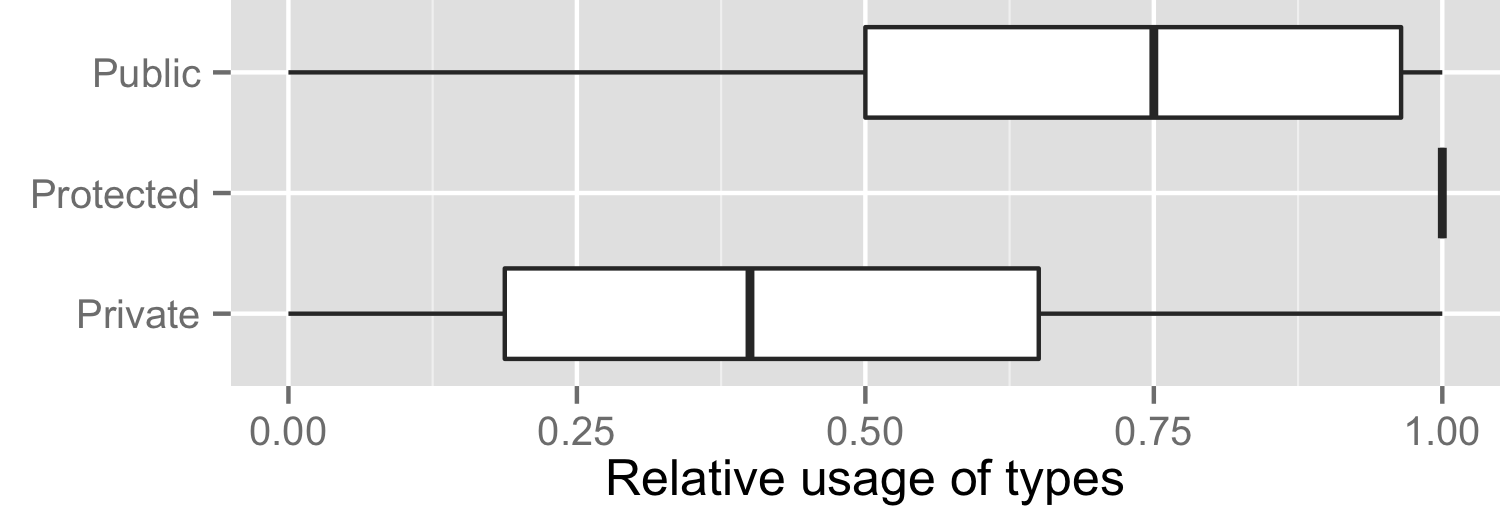
\includegraphics[width=0.45\textwidth]{../analysis/result/all/boxplots/23_declarations_by_visibility.png} 
\label{fig:all_boxplot_visibility_all} 

\vspace{0.3cm}

\renewcommand{\arraystretch}{1.2}
\small
\begin{tabular}{|c|c|c|c|c|}
\hline
Declaration Visibility	& n		& mean	& median	& std. dev.	\\
\hline
\hline
Public    				& 5852	& 0.69	& 0.75		& 0.29		\\ \hline
Protected 				& 2387	& 0.93	& 1.00		& 0.19		\\ \hline
Private   				& 6023	& 0.43	& 0.40		& 0.32		\\ \hline
\end{tabular}
\caption{Usage of types in all declarations by type of declaration}
\end{figure}


\begin{table}[h]

\centering{}%
\renewcommand{\arraystretch}{1.2}

\begin{tabular}{|c|c|c|c|}
\hline 
								& {}		& p		& conf. interval	\\
\hline
\hline
\multirow{2}{*}{Public}			& Protected	& 0.0000 & (-0.22,-0.18)	\\ 
								& Private	& 0.0000 &  (0.28, 0.31)	\\
\hline  
\multirow{2}{*}{Protected}		& Public	& 0.0000 & (0.18,0.22)	\\
								& Private	& 0.0000 & (0.54,0.57)	\\
\hline  
\multirow{2}{*}{Private}		& Public	& 0.0000 & (-0.31,-0.28)	\\
								& Protected	& 0.0000 & (-0.57,-0.54)	\\
\hline  
\end{tabular}
\label{tab:all_utest_visibility}
\caption{Mann-Whitney U Test results for the comparison between the usage of types by visibility of declaration}
\end{table}

Protected declarations are those typed most often.
Notice how skewed is the distribution for these elements in Figure \ref{fig:all_boxplot_visibility_all}.
Almost all 2387 projects which use protected visibility in their declarations type all of their protected fields, methods and constructors.
The confidence intervals reported by the U tests show a large difference between these declarations and those with either private or public visibility.
Although public declarations are not typed as much, they are also typed very often.
At least half of the projects type 75\% or more of their declarations.
Conversely private declarations are those with the smallest relative use of types.

% BREAKING VISIBILITY BY DECLARATION TYPE
% Figures \ref{fig:all_boxplot_visibility_methodReturn}-\ref{fig:all_boxplot_visibility_field} detail these results by declaration type.
% \begin{figure}[h]
% \centering 
% 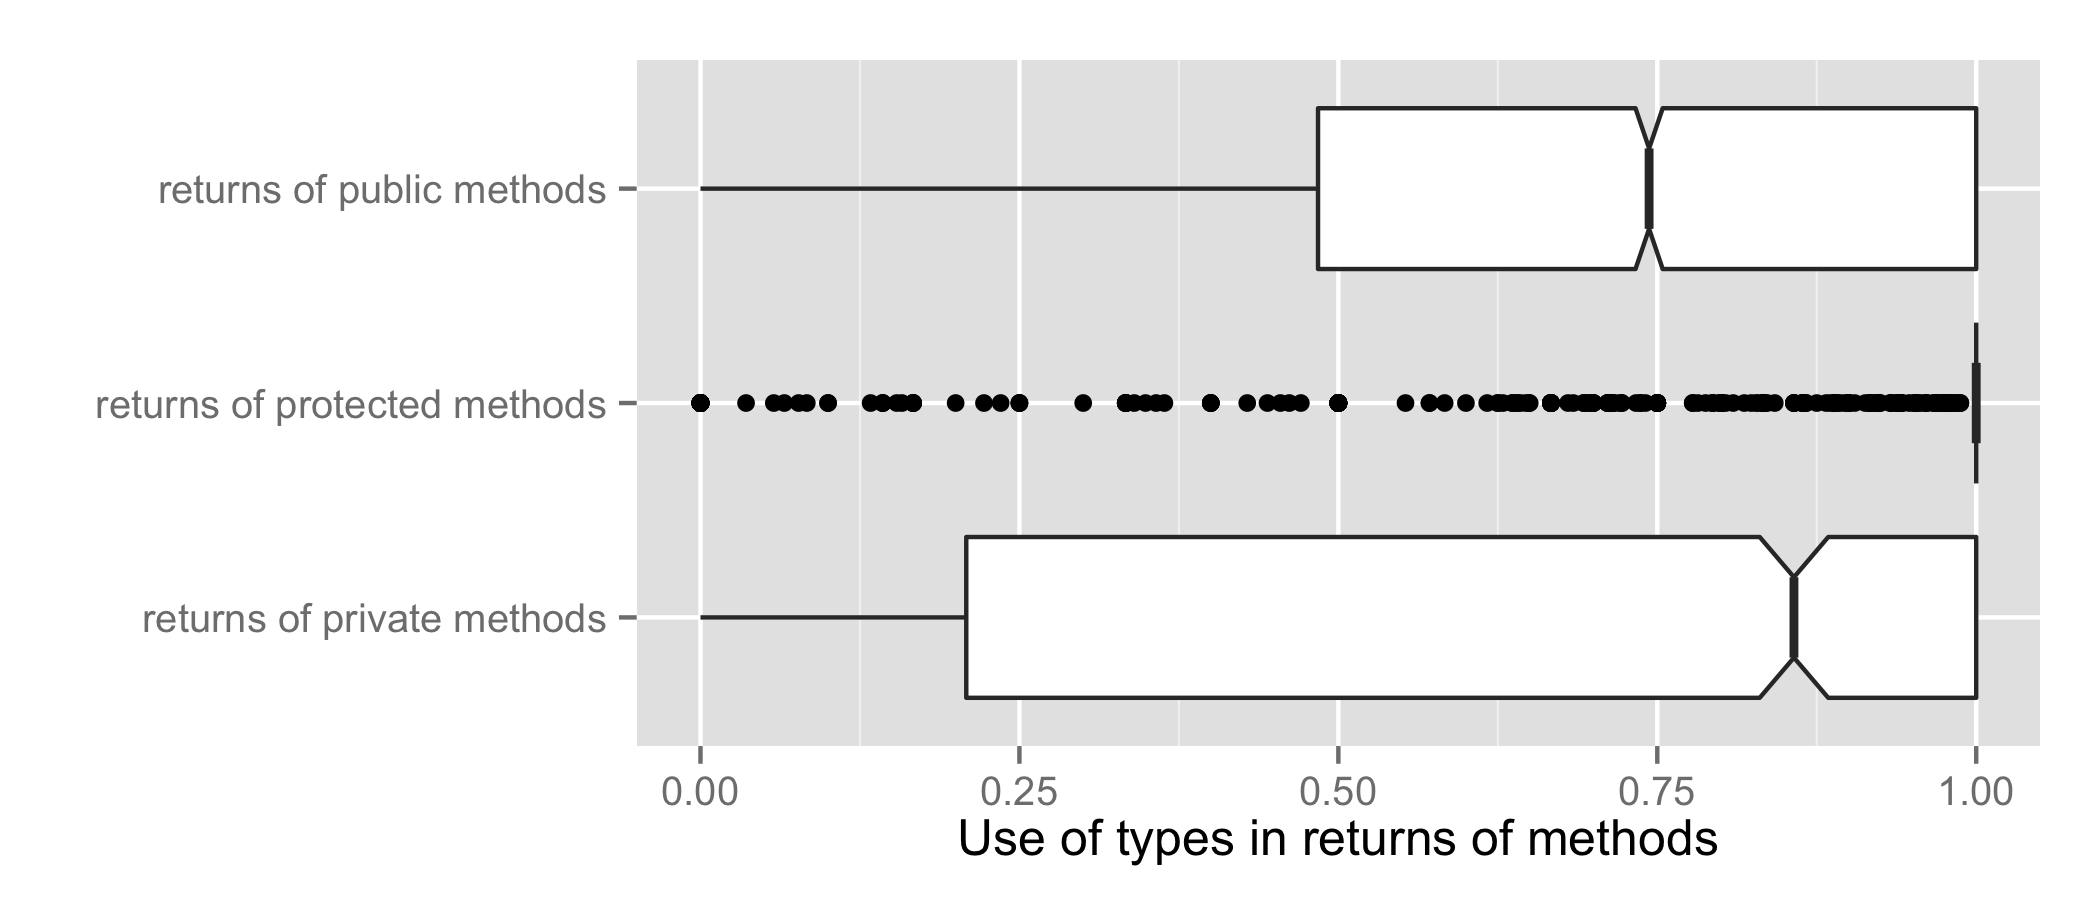
\includegraphics[width=0.45\textwidth]{../analysis/result/all/boxplots/11_returns_of_methods.png} 
% \caption{Usage of types in declarations of returns of methods by visibility}
% \label{fig:all_boxplot_visibility_methodReturn} 
% \end{figure}
% 
% \begin{figure}[h]
% \centering 
% 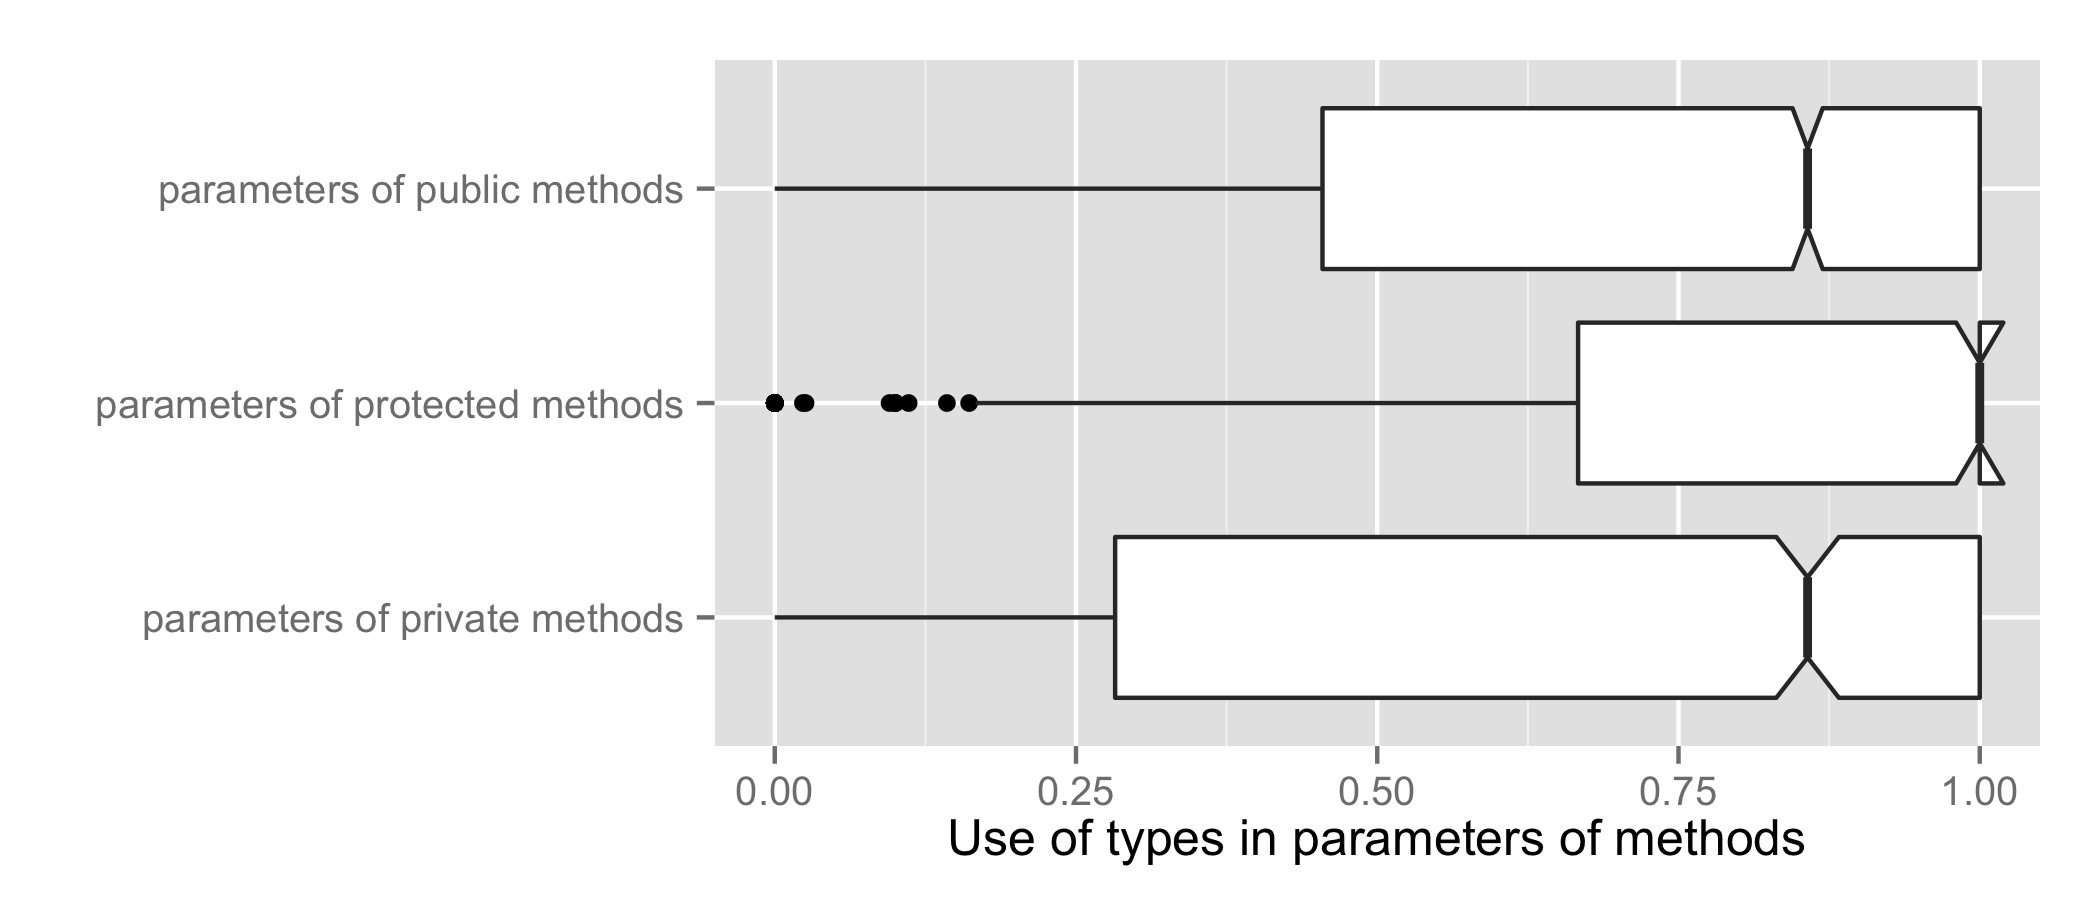
\includegraphics[width=0.45\textwidth]{../analysis/result/all/boxplots/14_parameters_of_methods.png} 
% \caption{Usage of types in declarations of parameters of methods by visibility}
% \label{fig:all_boxplot_visibility_methodParameter} 
% \end{figure}
% 
% \begin{figure}[h]
% \centering 
% 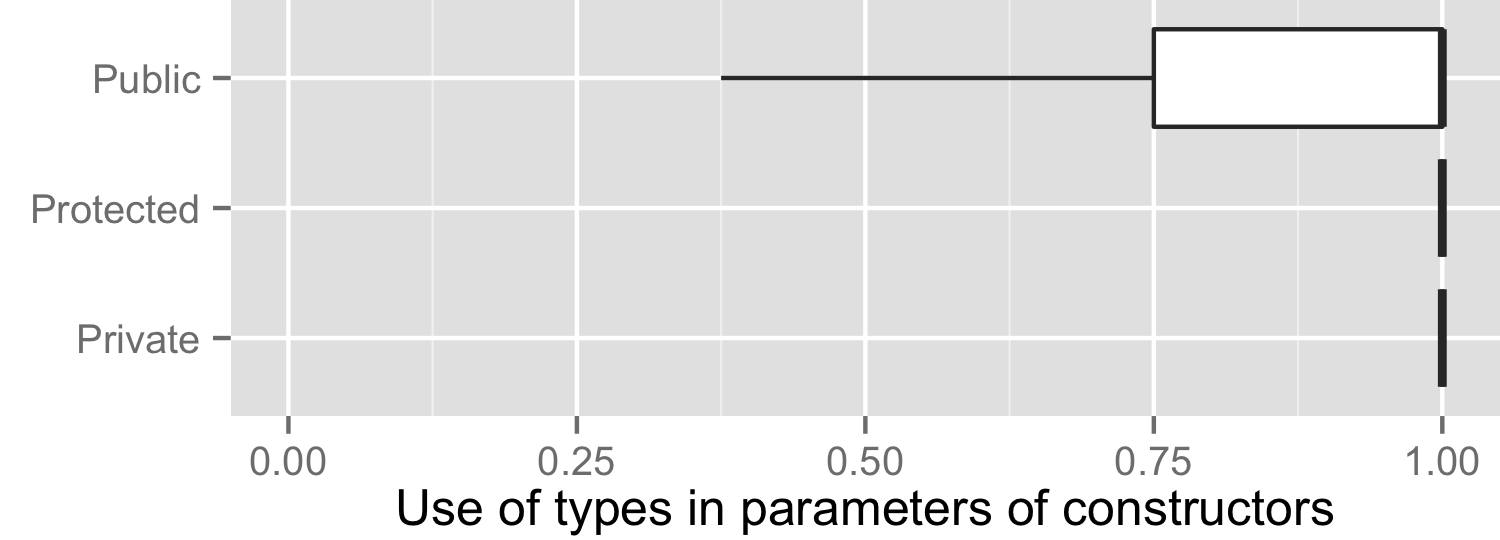
\includegraphics[width=0.45\textwidth]{../analysis/result/all/boxplots/17_parameters_of_constructors.png} 
% \caption{Usage of types in declarations of constructor parameters by visibility}
% \label{fig:all_boxplot_visibility_constructorParameter} 
% \end{figure}
% 
% \begin{figure}[h]
% \centering 
% 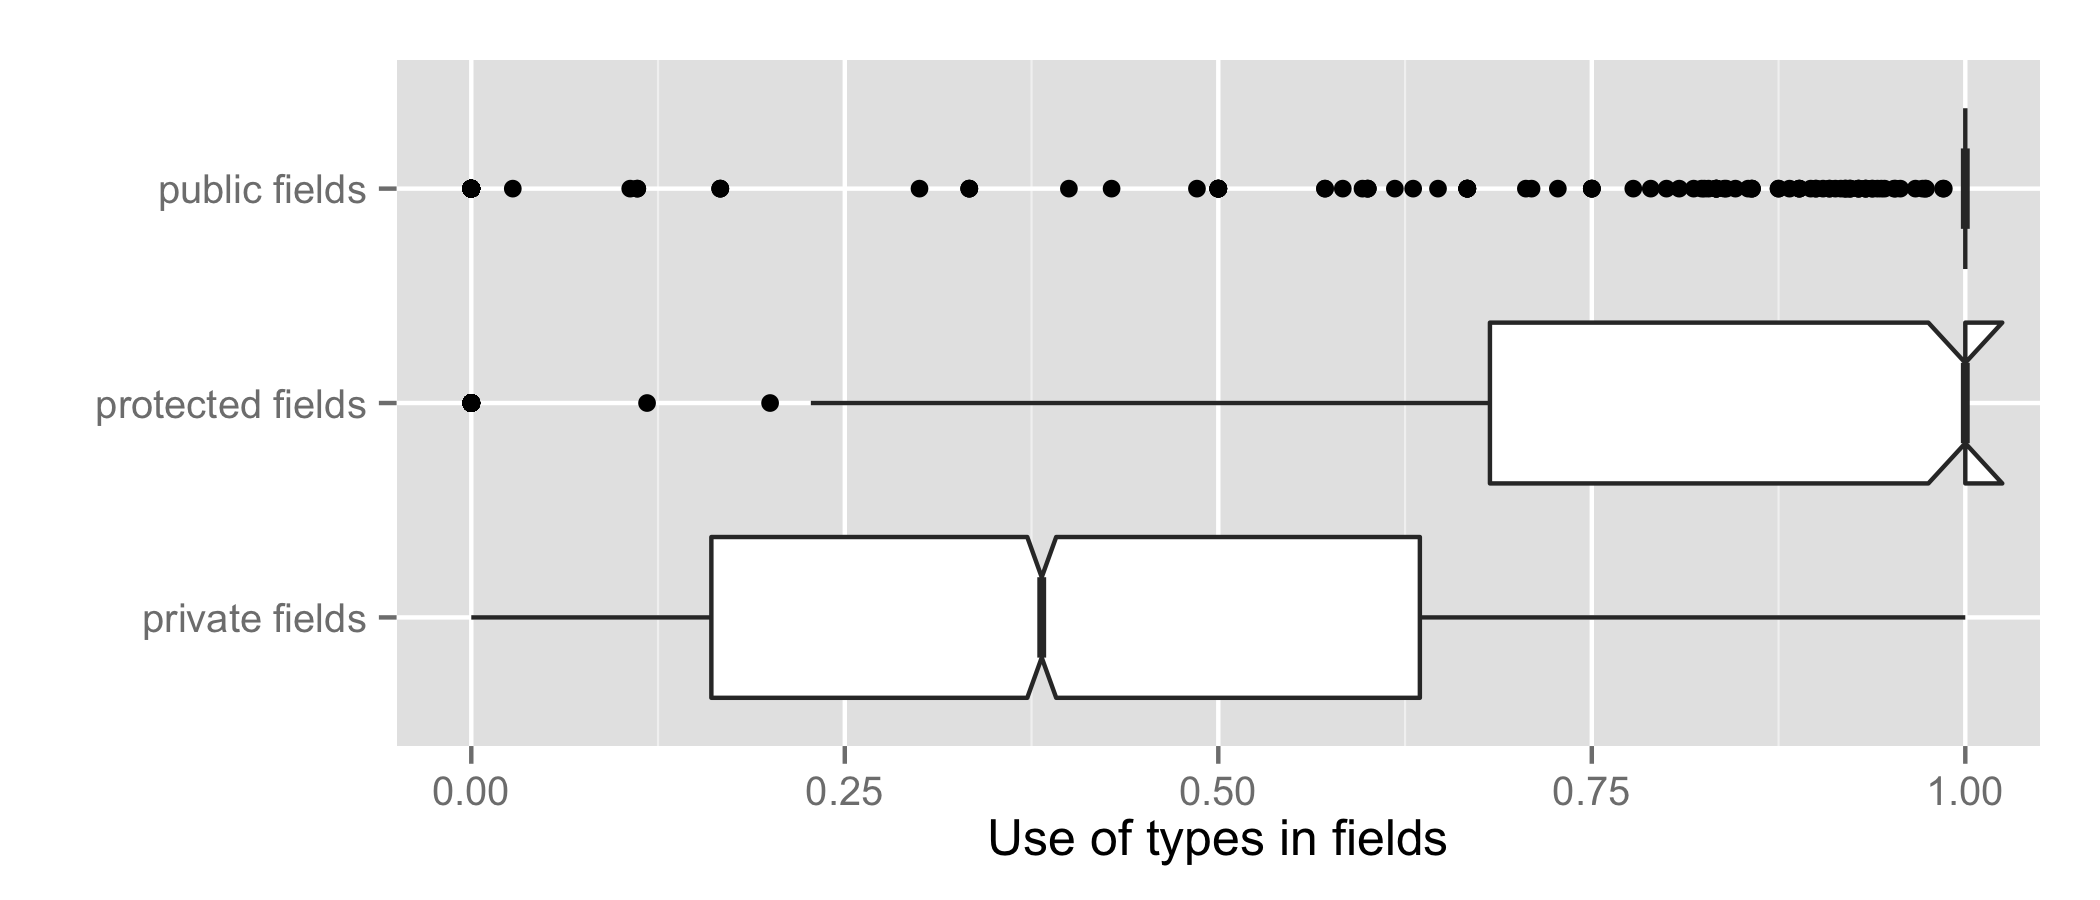
\includegraphics[width=0.45\textwidth]{../analysis/result/all/boxplots/20_fields.png} 
% \caption{Usage of types in declarations of fields by visibility}
% \label{fig:all_boxplot_visibility_field} 
% \end{figure}

% TESTS
\subsection{Test Classes and Main Classes\label{res-test-scripts}}
This sections investigates whether programmers type their declarations differently when they are writing test code.
A comparison between the usage of types in different declarations is shown in Figure \ref{fig:test_boxplot_type}. 
We also apply the Mann Whitney U test, but this time however we are not comparing declaration types to each other.
Instead, we are comparing declarations from main classes and test classes.
Results for the U test are shown in Table \ref{tab:test_utest_type}.
% Why not visibility
% TODO exaplin better how I segmented the data
% How do you identify test classes? Is a main class anything that is not a
% test class? What is a script?

There is no significant difference in the usage of types in fields and constructor parameters across test classes and main classes.
The p value reported by the U test comparing constructor parameters data is too high, 0.397, which does not allow us to reject the null hypothesis for this type of declaration.
As for fields, p value for the test comparing fields is small enough, 0.002, but the reported confidence interval negligible.

Local variables and method parameters are significantly less typed in test classes.
The confidence intervals reported in Table \ref{tab:test_utest_type} show a difference of (-0.500, -0.389) and (-0.058, -0.030) respectively, both with p-value equal to 0.
Method returns on the other hand are significantly more typed.
Figure \ref{fig:test_boxplot_type} shows a median equal to 1.00, which means that at least half of the projects type all of their method returns.
Although counter intuitive this result can be easily explained.
Automated testing frameworks usually enforce a certain method signature for test methods.
JUnit for example, which is used in 2525 out of the 5299 projects with test classes, requires the type of the return of a test methods to be \emph{void}.
Other popular test frameworks, such as TestNG, have similar requirements.
This means that, in this case, developers type their methods not because they want to, but because they need to.

\begin{figure}[h]
\centering 
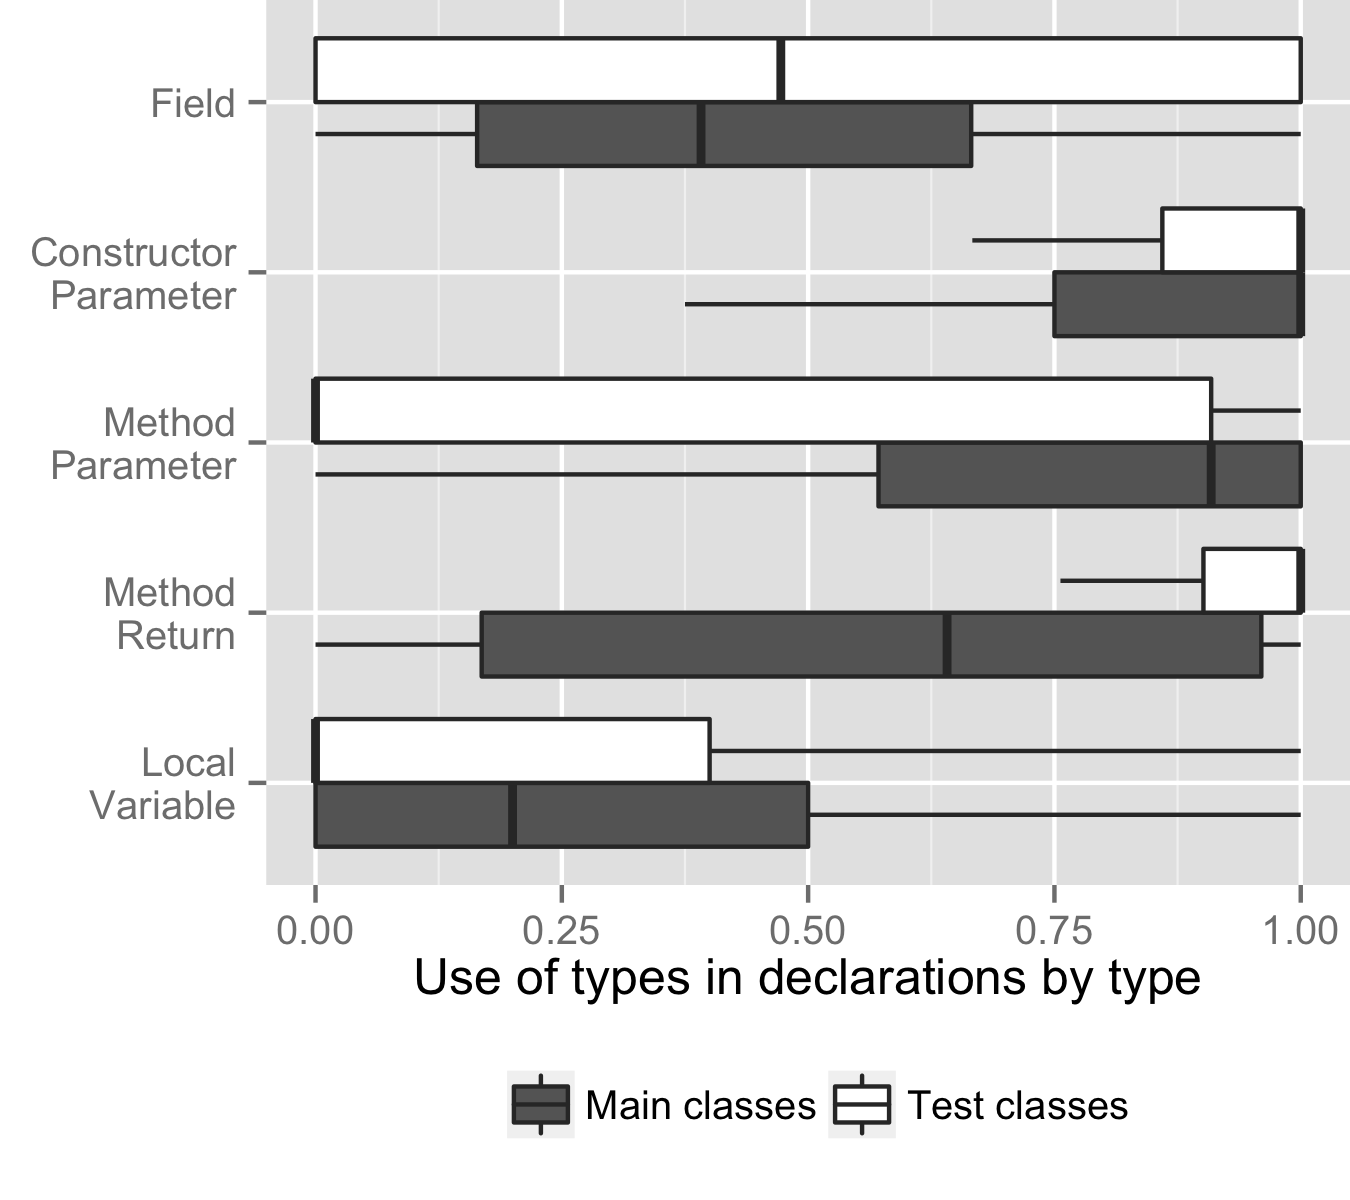
\includegraphics[width=0.45\textwidth]{../analysis/result/test/comparison/boxplots/6_declarations_by_type.png} 
\vspace{0.1cm}
\renewcommand{\arraystretch}{1.2}
\small
\raggedleft
\begin{tabular}{|c|c|c|c|c|c|}
\hline
\cell{Declaration\\Type}	& \cell{Class\\Type}& n		& mean		& median	& \cell{std.\\dev.}\\
\hline
\hline
\multirow{2}{*}{Field}	& Test			& 1778	& 0.48 		& 0.47	& 0.43 \\                
                			& Main			& 5857	& 0.43 		& 0.39	& 0.33 \\
\hline                
Constructor 			& Test			&  130	& 0.77 		& 1.00	& 0.40 \\                
Parameter				& Main			& 1623	& 0.80 		& 1.00	& 0.34 \\                
\hline
Method      			& Test			& 1546	& 0.34 		& 0.00	& 0.44 \\                
Parameter				& Main			& 4593	& 0.71 		& 0.91	& 0.35 \\                
\hline
Method      			& Test			& 4348	& 0.84 		& 1.00	& 0.31 \\                
Return		         	& Main			& 5299	& 0.54 		& 0.60	& 0.39 \\                
\hline
Local				& Test			& 2896	& 0.23 		& 0.00	& 0.35 \\                
Variable	        		& Main			& 5548	& 0.30 		& 0.19	& 0.32 \\                
\hline
\end{tabular}

\label{fig:test_boxplot_type} 
\caption{Usage of types by declaration type in test classes and main classes}
\end{figure}

\begin{table}[h!]
\centering{}%
\begin{tabular}{|c|c|c|}
\hline 
Declaration Type 		& p & conf. interval \\
\hline 
\hline 
Field                             & 0.0020		& (0.000, 0.000) \\ \hline
Constructor Parameter  & 0.3968	& (0.000, 0.000) \\ \hline
Method Parameter         & 0.0000	& (-0.519, -0.409) \\ \hline
Method Return              & 0.0000	& (0.200, 0.250) \\ \hline
Local Variable               & 0.0000		& (-0.070, -0.032) \\ 
\hline 
\end{tabular}
\label{tab:test_utest_type}
\caption{Mann-Whitney U Test results for the comparison between the usage of types by test classes and main classes}
\end{table}

% SCRIPTS
\subsection{Script Files and Class Files\label{res-test-scripts}}
We now analyze how programmers type their code in script files.
Figure \ref{fig:script_boxplot_type} shows the relative usage of types in declarations of local variables and parameters and returns of methods.
Constructors and fields are omitted since there is no way to declare those elements in scripts.
Table \ref{tab:script_utest_all} shows the results of the Mann-Whitney U test for these elements.
% Why not visibility
% When you compare classes to scripts, do you include test classes?

\begin{figure}[h]
\centering 
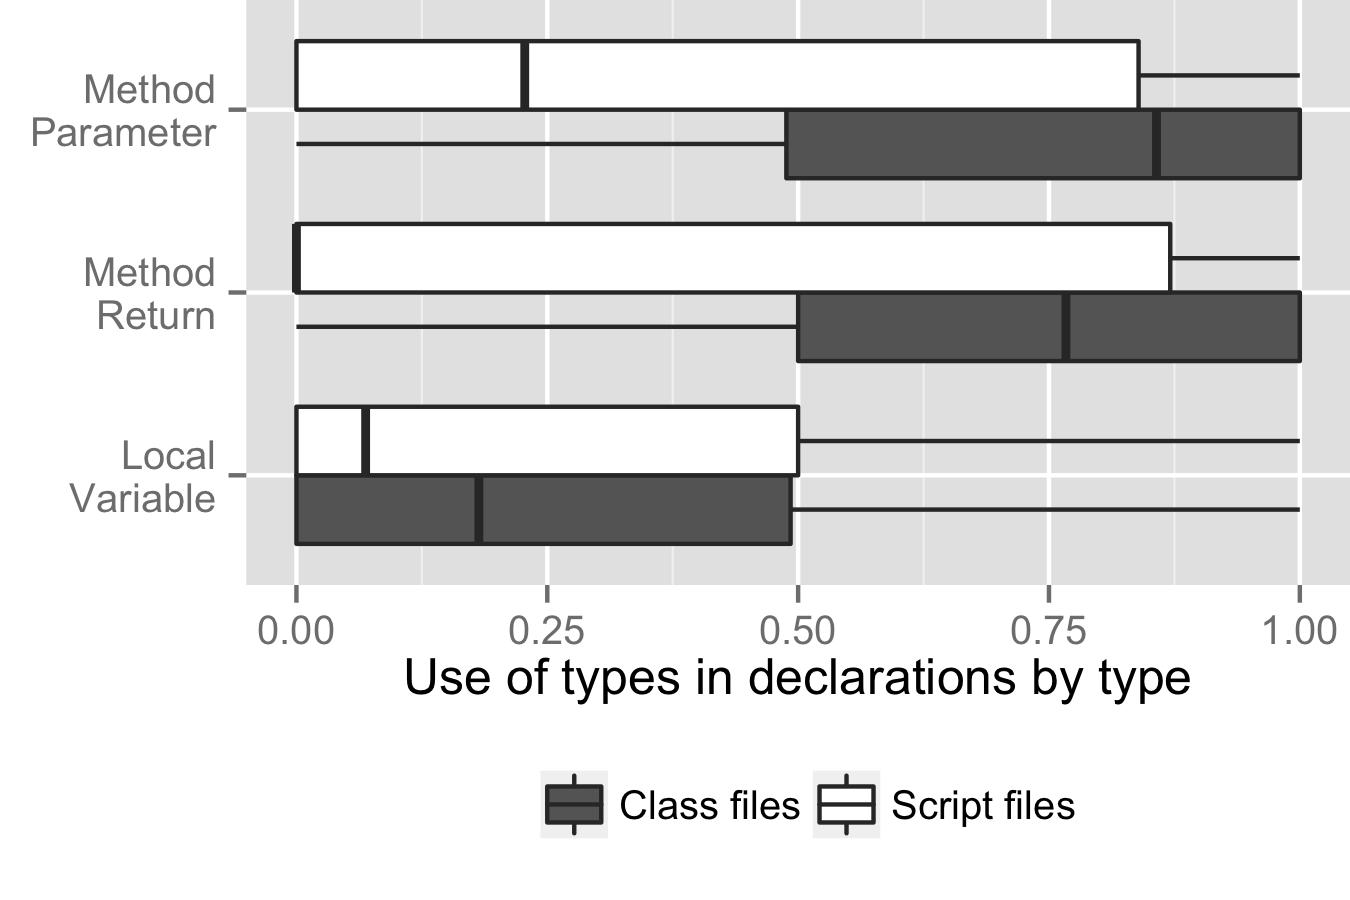
\includegraphics[width=0.45\textwidth]{../analysis/result/script/comparison/boxplots/6_declarations_by_type.png} 
\vspace{0.1cm}
\renewcommand{\arraystretch}{1.2}
\small
\raggedleft
\begin{tabular}{|c|c|c|c|c|c|}
\hline
\cell{Declaration\\Type}&\cell{File\\Type}	& n		& mean		& median	& \cell{std.\\dev.}\\
\hline
\hline
\hline	
Method					& Script			& 504 	& 0.40	& 0.23	& 0.42	 \\                
Parameter					& Class				& 4647	& 0.69	& 0.86	& 0.35	 \\                \hline	
Method					& Script			& 583 	& 0.34	& 0.00	& 0.43	 \\                
Return					& Class				& 5662	& 0.70	& 0.77	& 0.30	 \\                \hline	
Local					& Script			& 1775	& 0.28	& 0.07	& 0.37	 \\                
Variable	 				& Class				& 5246	& 0.30	& 0.18	& 0.32	 \\                
\hline
\end{tabular}
\caption{Usage of types by declaration type in script files and class files}
\label{fig:script_boxplot_type} 
\end{figure}

The p value for all executions of the U test is equal to 0, allowing to reject the null hypothesis.
The reported confidence interval for local variables however is too small and it can be argued that the difference in how programmers type these variables in scripts is insignificant.
On the other hand, parameters and returns of methods present a very different behavior.
Different from classes, most of projects do not type these declarations very often in scripts.
This is even more clear in method returns, where most of projects do not type any of these declarations.
Note however that the value for the last quartile of these elements is very high, superior to 0.8.
This indicates that there are a few projects that consistently type most of these declarations too.

\begin{table}[ht]
\centering{}%
\begin{tabular}{|c|c|c|}
\hline 
Declaration Type & p & conf. interval \\
\hline 
\hline 
Method Parameter              & 0.000	& (-0.365, -0.250) \\ \hline
Method Return                 & 0.000	& (-0.500, -0.414) \\ \hline
Local Variable                & 0.000	& (-0.016, 0.000)  \\ \hline
\hline 
\end{tabular}
\label{tab:script_utest_all}
\caption{Mann-Whitney U Test results for the comparison between the usage of types by script files and class files}
\end{table}

% PROGRAMMERS BACKGROUND
\subsection{Programmers' Background\label{res-background}}
In this section, we analyze how programmers use types in their declarations according to their backgrounds.
Projects are distributed in three groups based on the type system of the languages their developers have used on GitHub.
The first group contains those projects of programmers who developed only in statically typed languages, such as Java or C\#.
The projects of those who developed only in dynamically typed languages, such as Ruby or JavaScript, comprise the second group.
Finally, the third group includes the project of those programmers with both dynamically and statically typed languages in their portfolio.
Figures \ref{fig:background_boxplot_type} and \ref{fig:background_boxplot_visibility}  show results by declaration type and visibility respectively.
Results for the Mann-Whitney U test are reported in Tables \ref{tab:background_utest_type} and \ref{tab:backgorund_utest_visibility}.
Notice that these tables are divided in three groups, each one corresponding to the comparison between the data for the three different background groups.

\begin{figure}[h]
\centering 
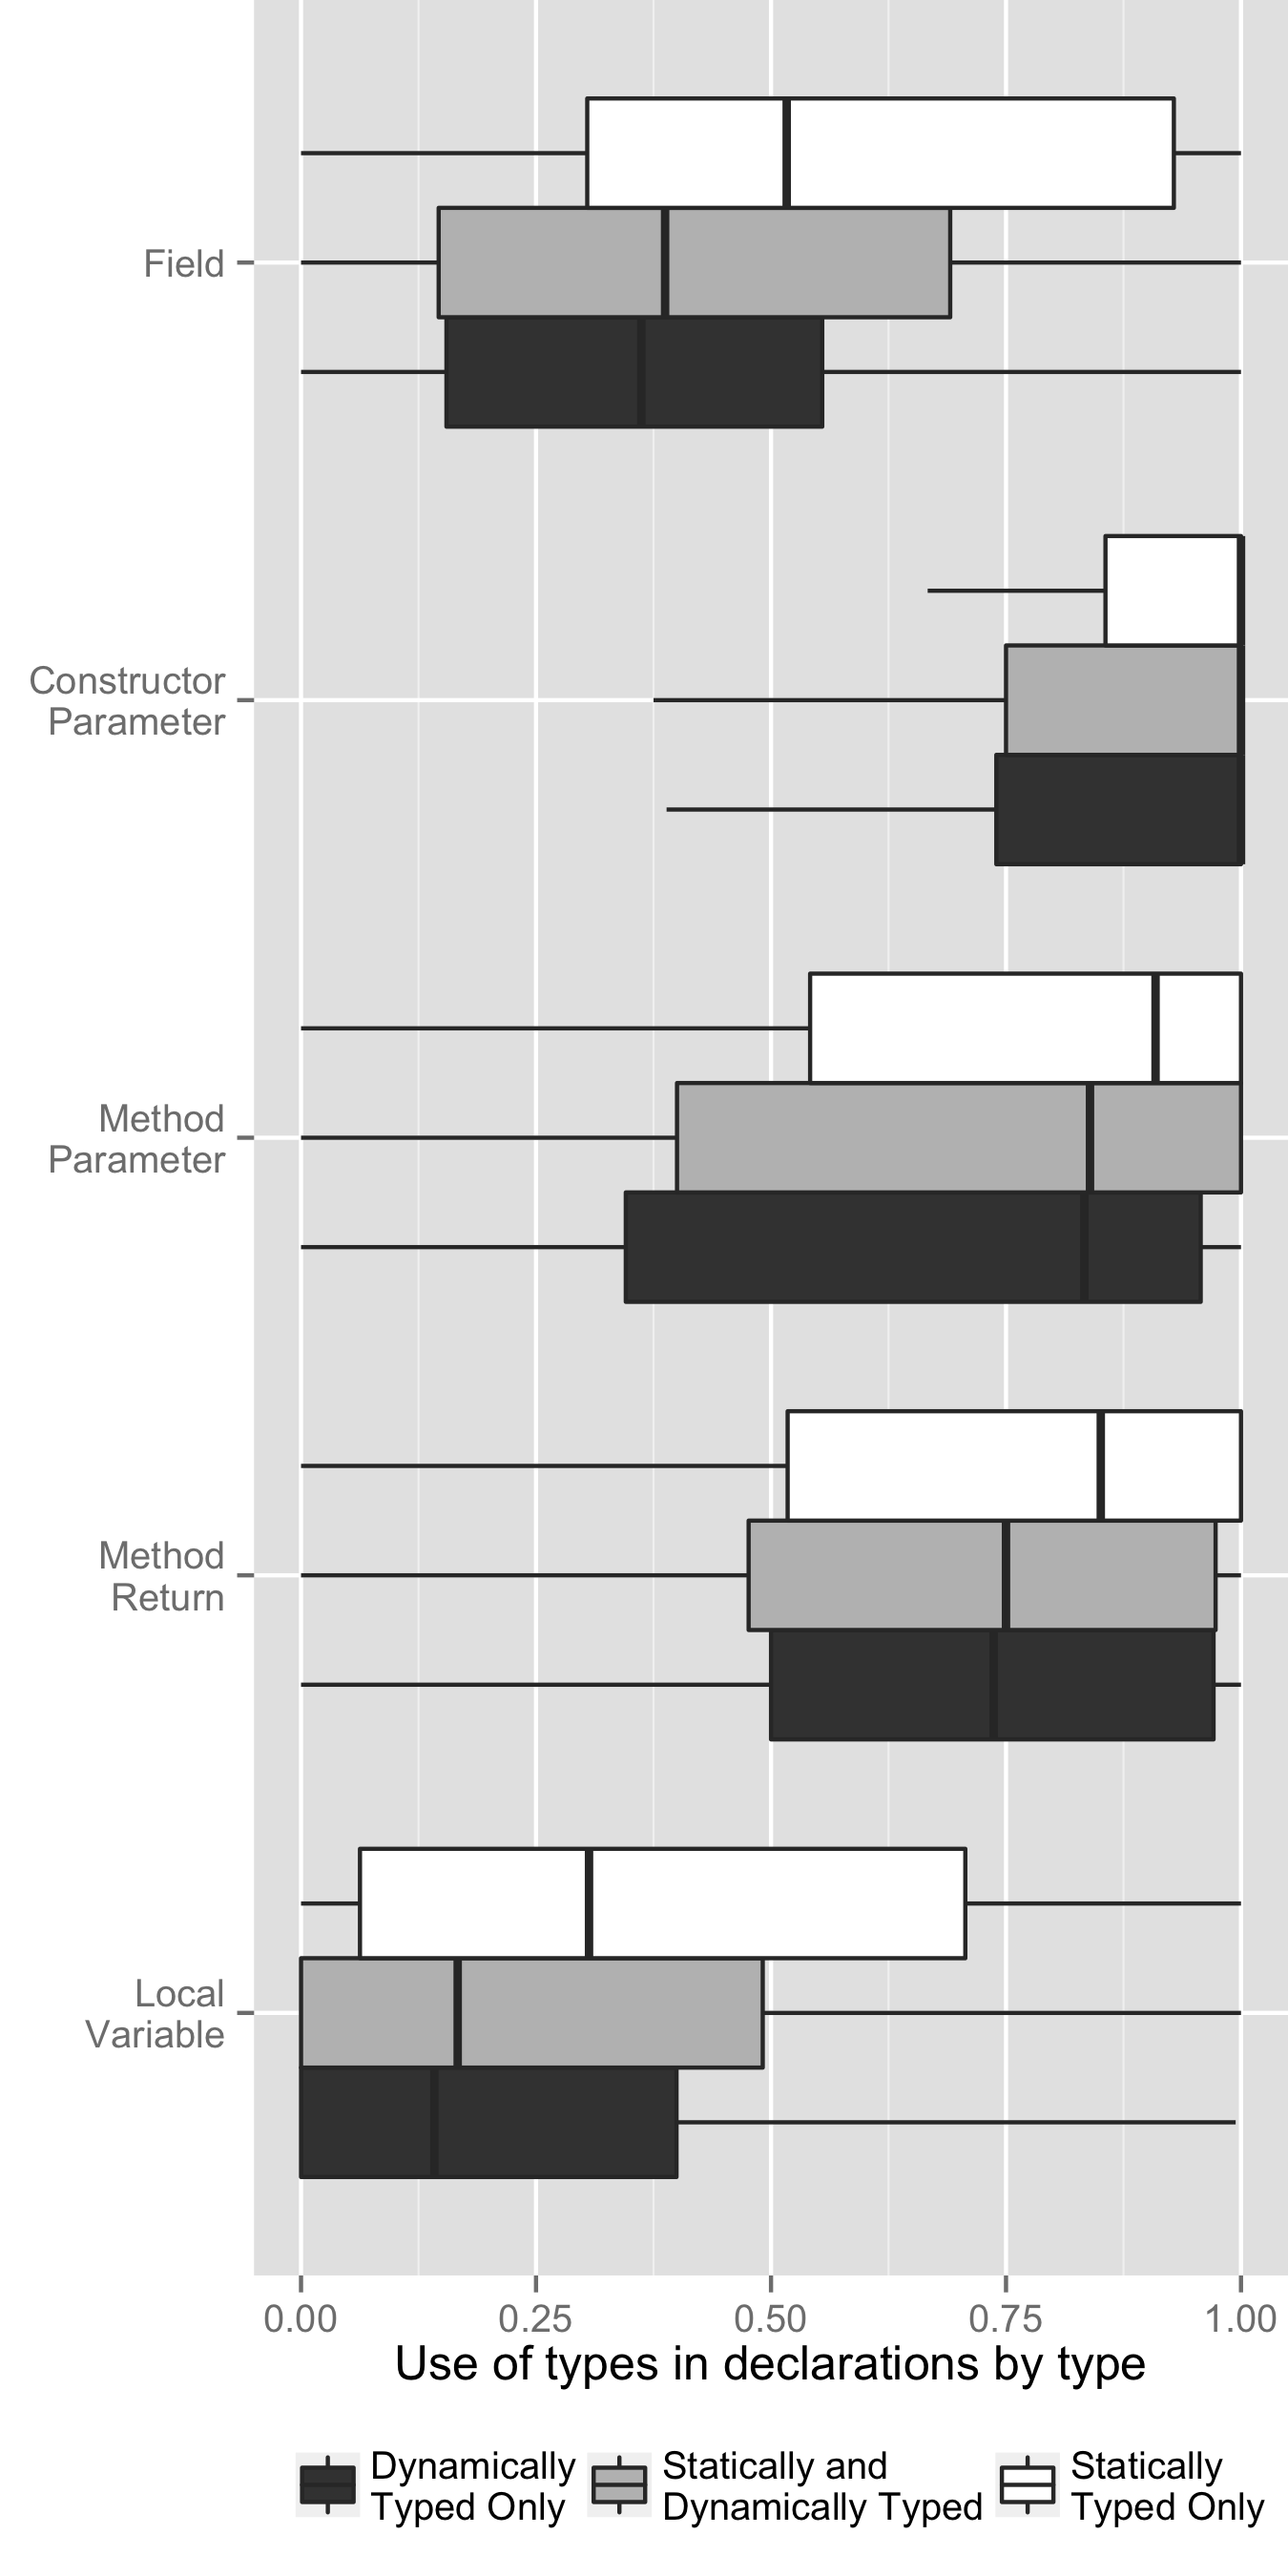
\includegraphics[width=0.45\textwidth]{../analysis/result/background/comparison/boxplots/6_declarations_by_type.png} 
\vspace{0.1cm}
\renewcommand{\arraystretch}{1.2}
\small
\raggedleft
\begin{tabular}{|c|c|c|c|c|c|}
\hline
\cell{Declaration\\Type}						& \cell{Background}	& n		& mean		& median	& \cell{std.\\dev.}\\
\hline
\hline
{}												& Static			& 782	& 0.56		& 0.52 		& 0.35\\			 
Field											& Both				& 3183	& 0.43		& 0.39 		& 0.34\\			 
{}												& Dynamic			& 2035	& 0.38		& 0.36 		& 0.29\\
\hline								 			
\multirow{3}{*}{\cell{Constructor\\Parameter}}	& Static			& 224	& 0.83		& 1.00 		& 0.33\\			 
												& Both				& 991	& 0.80		& 1.00 		& 0.35\\			 
												& Dynamic			& 455	& 0.80		& 1.00 		& 0.34\\			 
\hline								
\multirow{3}{*}{\cell{Method\\Parameter}}		& Static			& 662	& 0.73		& 0.91 		& 0.34\\			 
												& Both				& 2694	& 0.67		& 0.84 		& 0.36\\			 
												& Dynamic	 		& 1511	& 0.65		& 0.83 		& 0.37\\	
\hline						 			
\multirow{3}{*}{\cell{Method\\Return}}			& Static			& 764	& 0.73		& 0.85 		& 0.30\\			 
												& Both				& 3205	& 0.66		& 0.75 		& 0.32\\			 
												& Dynamic	 		& 1912	& 0.68		& 0.74 		& 0.29\\ 
\hline											
\multirow{3}{*}{\cell{Local Variable}}			& Static			& 798	& 0.39		& 0.31 		& 0.36\\			 
												& Both				& 3230	& 0.28		& 0.17 		& 0.32\\			 
												& Dynamic			& 1817	& 0.25		& 0.14 		& 0.30\\ 
\hline
\end{tabular}
\label{fig:background_boxplot_type}
\caption{Usage of types by declaration type and programmer background}
\end{figure}

                
\begin{figure}[ht]
\centering 
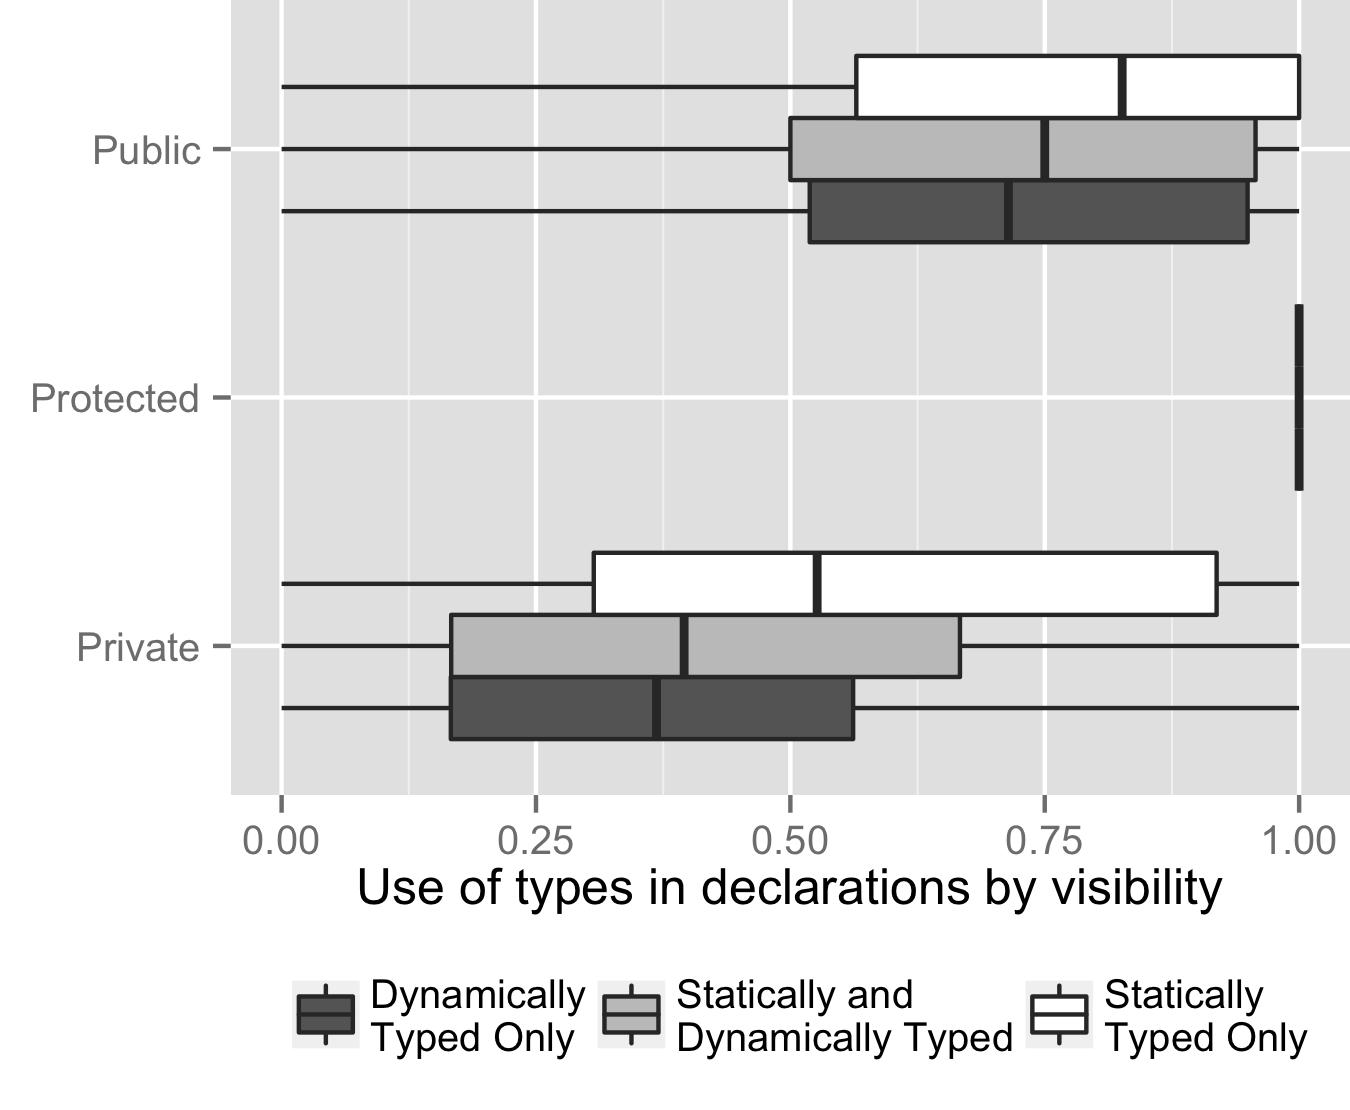
\includegraphics[width=0.45\textwidth]{../analysis/result/background/comparison/boxplots/23_declarations_by_visibility.png} 
\vspace{0.1cm}
\renewcommand{\arraystretch}{1.2}
\small
\raggedleft
\begin{tabular}{|c|c|c|c|c|c|}
\hline
\cell{Declaration\\Type}						& \cell{Background}	& n		& mean		& median	& \cell{std.\\dev.}\\
\hline
\hline
{}												& Static			& 757 	& 0.73		& 0.83 		& 0.29\\			 
Public											& Both				& 3191	& 0.68		& 0.75 		& 0.30\\			 
{}												& Dynamic			& 1904	& 0.69		& 0.71 		& 0.27\\
\hline								 								    	    		    		    						
\multirow{3}{*}{\cell{Protected}}				& Static			& 287 	& 0.92		& 1.00 		& 0.20\\			 
												& Both				& 1275	& 0.94		& 1.00 		& 0.18\\			 
												& Dynamic			& 825 	& 0.93		& 1.00 		& 0.20\\			 
\hline																    	    		    		    					
\multirow{3}{*}{\cell{Private}}					& Static			& 787 	& 0.56		& 0.53 		& 0.34\\			 
												& Both				& 3196	& 0.43		& 0.40 		& 0.33\\			 
												& Dynamic	 		& 2040	& 0.38		& 0.37 		& 0.28\\	
\hline						 			
\end{tabular}
\label{fig:background_boxplot_visibility}
\caption{Usage of types by declaration visibility and programmer background}
\end{figure}	

\begin{table}[h!]
\centering{}%
\renewcommand{\arraystretch}{1.2}

\begin{tabular}{|c|c|c|c|}
\hline 
{}															& Declaration Type 		& p 		& conf. interval \\
\hline 
\hline 
\multirow{5}{*}{\cell{Static\\vs.\\Static and\\Dynamic}}	& Field					& 0.0000	& (0.073, 0.163)	\\ \cline{2-4}
															& Constructor Parameter	& 0.7281	& (0.000, 0.000)	\\ \cline{2-4}
															& Method Parameter		& 0.0000	& (0.000, 0.036)	\\ \cline{2-4}
															& Method Return			& 0.0000	& (0.000, 0.067)	\\ \cline{2-4}
															& Local Variable		& 0.0000	& (0.038, 0.100)	\\ 
\hline 
\hline

\multirow{5}{*}{\cell{Static\\vs.\\Dynamic}}				& Field					& 0.0000	& (0.139, 0.228)	\\ \cline{2-4}
															& Constructor Parameter	& 0.9347	& (0.000, 0.000)	\\ \cline{2-4}
															& Method Parameter		& 0.0000	& (0.005, 0.076)	\\ \cline{2-4}
															& Method Return			& 0.0000	& (0.000, 0.062)	\\ \cline{2-4}
															& Local Variable		& 0.0000	& (0.057, 0.126)	\\ 
\hline 
\hline
\multirow{5}{*}{\cell{Static and\\Dynamic\\vs.\\Dynamic}}	& Field					& 0.0000	& (0.000, 0.050)	\\ \cline{2-4}
															& Constructor Parameter	& 0.7531	& (0.000, 0.000)	\\ \cline{2-4}
															& Method Parameter		& 0.0032	& (0.000, 0.013)	\\ \cline{2-4}
															& Method Return			& 0.5269	& (0.000, 0.000)	\\ \cline{2-4}
															& Local Variable		& 0.0071	& (0.000, 0.005)	\\ 
\hline 
\end{tabular}
\label{tab:background_utest_type}
\caption{Mann-Whitney U Test results for the comparison between the usage of types by declaration type and programmers background}
\end{table}
      
\begin{table}[h!]
\centering{}%
\renewcommand{\arraystretch}{1.2}
\begin{tabular}{|c|c|c|c|}
\hline 
{}															& Declaration Visibility 	& p 		& conf. interval \\
\hline 
\hline 
\multirow{3}{*}{\cell{Static vs.\\Static and\\Dynamic}}		& Public					& 0.0000	& (0.000, 0.058)	\\ \cline{2-4}
															& Protected					& 0.1287	& (0.000, 0.000)	\\ \cline{2-4}
															& Private					& 0.0000	& (0.082, 0.167)	\\ 
\hline 
\hline

\multirow{3}{*}{\cell{Static\\vs.\\Dynamic}}				& Public					& 0.0000	& (0.000, 0.065)	\\ \cline{2-4}
															& Protected					& 0.1130	& (0.000, 0.000)	\\ \cline{2-4}
															& Private					& 0.0000	& (0.143, 0.229)	\\ 
\hline 
\hline
\multirow{3}{*}{\cell{Static and\\Dynamic vs.\\Dynamic}}	& Public					& 0.0000	& (0.000, 0.051)	\\ \cline{2-4}
															& Protected					& 0.8260	& (0.000, 0.000)	\\ \cline{2-4}
															& Private					& 0.8328	& (0.000, 0.000)	\\ 
\hline 
\end{tabular}
\label{tab:backgorund_utest_visibility}
\caption{Mann-Whitney U Test results for the comparison between the usage of types by declaration visibility and programmers background}
\end{table}
              
The usage of types by programmers with both statically and dynamically typed languages in their portfolio is similar to that of programmers with dynamically languages only.
According to Tables \ref{tab:background_utest_type} and \ref{tab:backgorund_utest_visibility}, the only significant differences in the usage of types are in  declarations of fields or in those with public visibility.
Still, the confidence interval is arguably small, between 0 and 0.051 in both cases.
Conversely, programmers with only statically typed languages in their portfolio tend to use types more often than others.
There are only two situations where the p value reported by the Mann-Whitney U test is big enough so the null hypothesis can not be rejected, protected declarations and declarations of constructor parameters.
% Discuss a little bit more and add some conclusions



% PROJECT MATURITY
\subsection{Project Maturity\label{res-size}}
% TODO: Discuss mature selection and mitigate threatens
% You mention that some clearly mature projects are only 2K lines of code or
% have only 100 commits. But would a 100 000 line project with only 100
% commits be considered mature?
% It is surprising that from over 7000 projects, only 203 have both more than
% 2000 lines and 100 commits. Why is that?


This section investigates whether programmers use types differently in their code depending on the project maturity.
Three metrics are used to define the maturity of the project: age, number lines of code and number of commits.
We start by analyzing the correlation between these metrics and the relative use of types in declarations by type and visibility.
The Spearman rank correlation coefficient is used for this purpose.
This coefficient, which can go from -1 to 1, is a measure of the dependence between two variables.
A positive value means that, as the valuable of one variable grows, so does the value of the other.
A negative value means the opposite.
Values close to 1 or -1 indicate very strong relationships while values above 0.5 or below -0.5 can be considered strong correlations.

\begin{table}[h!]
\centering{}%
\begin{tabular}{|c|c|c|c|c|}
\hline 
Declaration Type/Visibility	& Size		& Age	&	Commits\\
\hline 
\hline 
Field						&  0.221	& -0.063	&  0.153	\\ \hline
Constructor Parameter		& -0.072	& -0.132	& -0.053	\\ \hline
Method Parameter			& -0.123	& -0.079	& -0.004	\\ \hline
Method Return				& -0.071	&  0.168	& -0.027	\\ \hline
Local Variable		 		&  0.057	& -0.049	&  0.112	\\ 
\hline 			 
\hline 		 
Public						& -0.063	&   0.119	& -0.024	\\ \hline
Protected					& -0.286	&  -0.020	& -0.165	\\ \hline
Private				 		&  0.213	&  -0.068	&  0.160	\\ \hline
\end{tabular}
\label{tab:all_correlation_maturity}
\caption{Spearman Correlation between the usage of types and the size, age and number of commits of projects}
\end{table}	


Table \ref{tab:all_correlation_maturity} shows the Spearman correlation coefficient between the usage of types and the three metrics of maturity.
Most of values in this table are close to 0.
There are a few which could indicate a weak relationship, such as \emph{Size} vs. \emph{protected} or \emph{commits} vs. \emph{private}, but these values are too small and could have happened by chance.
Thus, we can not say that there is a correlation between the metrics of maturity and the usage of types.

% The project size is a simple metric to measure the complexity of a project.
% Usually, the larger the project, the greater the number of modules and the need for maintenance \cite{Fenton1998}. 

The lack of correlation does not necessarily imply that the maturity of a project has no influence on the usage of types.
This influence could appear only when the combination of the three metrics of maturity is big enough.
In order to understand if this is true, we conduct now a comparison between mature projects and the rest of the data.
In order for a project to be considered mature it has to have at least 2KLoC, 100 commits and be 100 days old.
These numbers were defined by manually inspecting our dataset and finding that there are popular and mature projects that barely exceed these three metrics.
According to our criteria, there are 223 mature projects in our dataset
These projects are detailed in Table \ref{tab:mature_dataset_characterization}.



\begin{table}[h!]

\centering{}%
\renewcommand{\arraystretch}{1.2}

\begin{tabular}{|c|c|c|c|c|c|}
\hline
{}		& mean	& median	& std. dev.	& max	& total		\\
\hline
\hline
Size (LoC)	& 9947 	& 5627 & 14594  & 149933	& 2218189	\\ \hline
Commits   	& 487  	& 213    & 800   & 6545		& 108583	\\ \hline
Age (Days)  & 600  	& 574  & 350   & 1469		& 133697	\\ \hline
\end{tabular}
\caption{Descriptive statistics for mature projects}
\label{tab:mature_dataset_characterization}
\end{table}

Figure \ref{fig:size_boxplot_type}  and \label{fig:size_boxplot_visibility} compares the usage of types between mature projects and others and Tables \ref{tab:size_utest_type} and \ref{tab:size_utest_visibility} show the results for the Mann-Whitney U test for these comparisons.
There are significant differences only in two declarations types, fields and local variables.
As for the visibility, only protected declarations can be said to be significantly different.
Note that for private declarations, the p-value is 0, but the confidence interval for the difference of medians is negligible.
% comment on these differences

\begin{figure}[h!]
\centering 
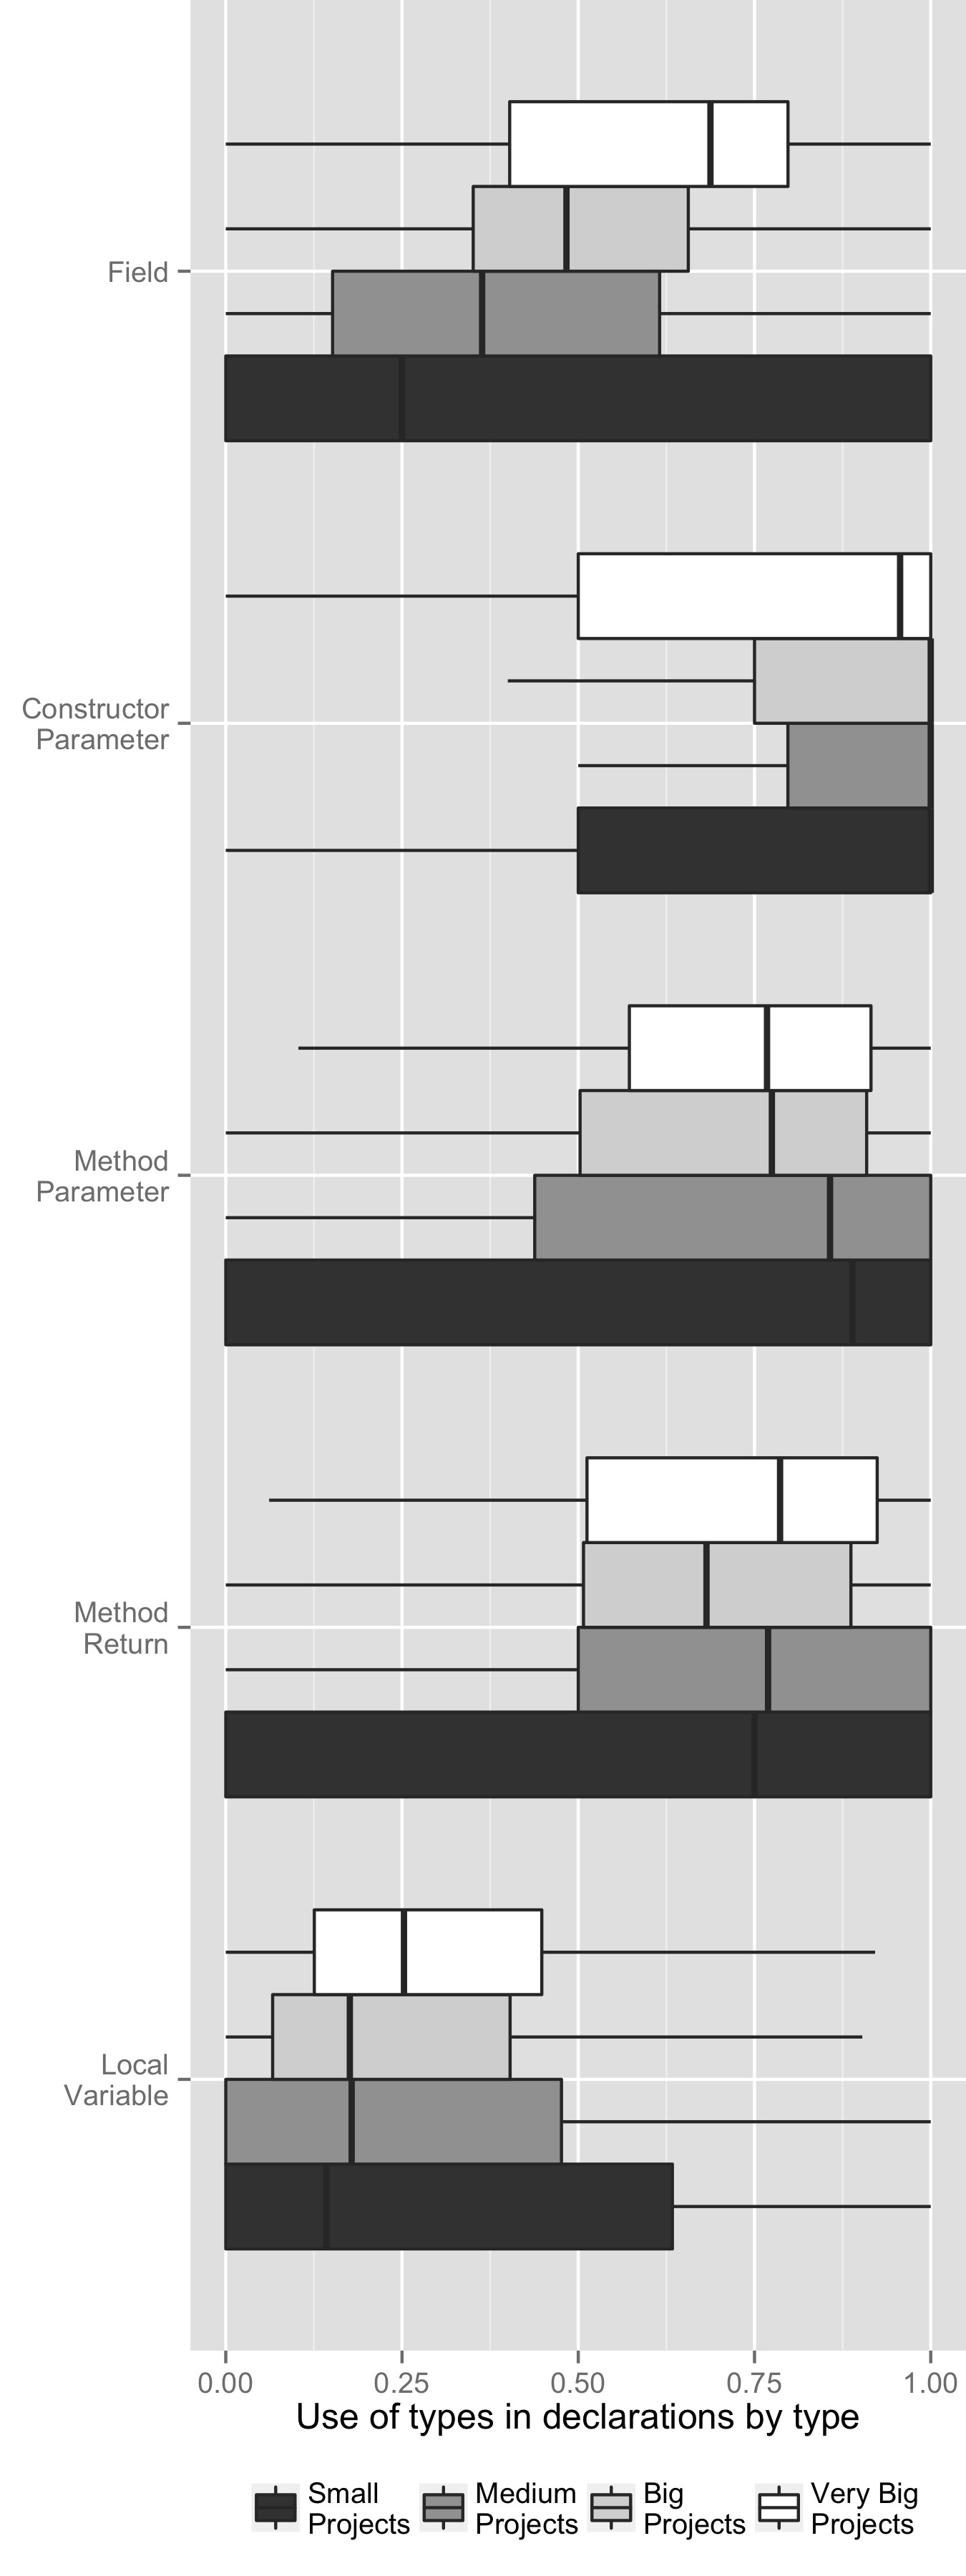
\includegraphics[width=0.45\textwidth]{../analysis/result/size/comparison/boxplots/6_declarations_by_type.png} 
\vspace{0.1cm}
\renewcommand{\arraystretch}{1.2}
\small
\raggedleft
\begin{tabular}{|c|c|c|c|c|c|}
\hline
\cell{Declaration\\Type}	& \cell{Project\\Type}& n	& mean	& median	& \cell{std.\\dev.}\\
\hline
\hline
\multirow{2}{*}{Field}		& Other			& 5779	& 0.43 		& 0.39	& 0.33 \\                
                			& Mature		& 221 	& 0.53 		& 0.48	& 0.27 \\
\hline                																								
Constructor 				& Other			& 1498	& 0.80 		& 1.00	& 0.35 \\                
Parameter					& Mature		& 172 	& 0.83 		& 1.00	& 0.30 \\                
\hline																								
Method      				& Other			& 4645	& 0.67 		& 0.86	& 0.37 \\                
Parameter					& Mature		& 222 	& 0.69 		& 0.78	& 0.29 \\                
\hline																								
Method						& Other			& 5659	& 0.68 		& 0.75	& 0.32 \\                
Return		         		& Mature		& 222 	& 0.72 		& 0.79	& 0.24 \\                
\hline																								
Local						& Other			& 5622 	& 0.29 		& 0.17	& 0.32 \\                
Variable					& Mature		& 223	& 0.32 		& 0.22	& 0.28 \\                
\hline																								
\end{tabular}
\label{fig:size_boxplot_type} 
\caption{Usage of types in projects by declaration type and project maturity}
\end{figure}


\begin{figure}[h!]
\centering 
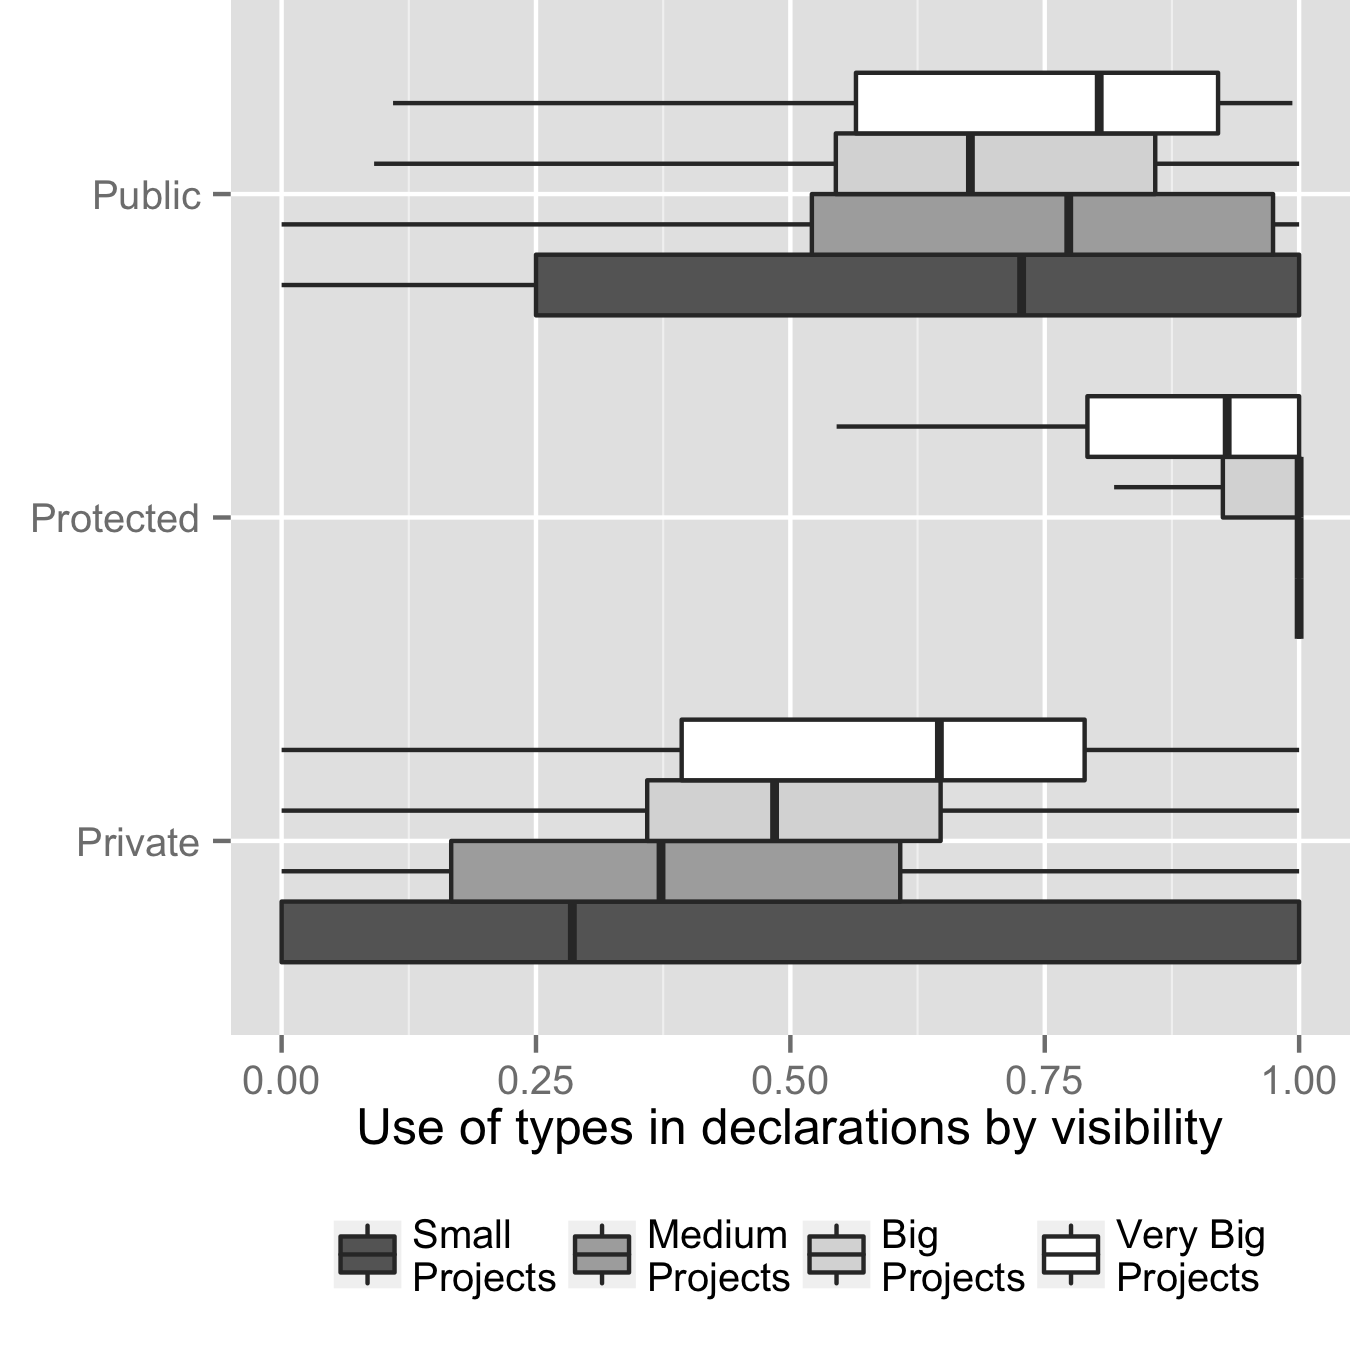
\includegraphics[width=0.45\textwidth]{../analysis/result/size/comparison/boxplots/23_declarations_by_visibility.png} 
\vspace{0.1cm}
\renewcommand{\arraystretch}{1.2}
\small
\raggedleft
\begin{tabular}{|c|c|c|c|c|c|}
\hline
\cell{Declaration\\Type}			& \cell{Project\\Type}	& n		& mean		& median	& \cell{std.\\dev.}\\
\hline
\hline
\multirow{2}{*}{\cell{Public}}		& Other					& 5629	& 0.69		& 0.75 		& 0.29\\			 
{}									& Mature				& 223 	& 0.72		& 0.76 		& 0.24\\
\hline								 							  	  			  			  							
\multirow{2}{*}{\cell{Protected}}	& Other					& 2204	& 0.94		& 1.00 		& 0.19\\			 
									& Mature				& 183 	& 0.88		& 1.00 		& 0.21\\			 
\hline															  	  			  			  						
\multirow{2}{*}{\cell{Private}}		& Other					& 5802	& 0.43		& 0.40 		& 0.32\\			 
									& Mature				& 221 	& 0.53		& 0.48 		& 0.26\\			 
\hline						 			
\end{tabular}
\label{fig:size_boxplot_visibility}
\caption{Usage of types in projects by declaration visibility and project maturity}
\end{figure}	

\begin{table}[h!]
\centering{}%
\begin{tabular}{|c|c|c|}
\hline 
Declaration Type/Visibility 		& p & conf. interval \\
\hline 
\hline 
Field                  & 0.0000	& (0.053,0.173)	\\ \hline
Constructor Parameter  & 0.3203	& (0.000,0.000) \\ \hline
Method Parameter       & 0.0794	& (-0.051,0.002) \\ \hline
Method Return          & 0.9373	& (-0.031,0.051) \\ \hline
Local Variable         & 0.0002	& (0.012,0.078)	\\ \hline
\hline 
Public		& 0.8540	& (-0.031,0.045)	\\ \hline
Private		& 0.0000	& (0.000,0.000)		\\ \hline
Protected	& 0.0000	& (0.055,0.169)		\\ 
\hline 
\end{tabular}
\label{tab:size_utest_visibility}
\caption{Mann-Whitney U Test results for the comparison between the usage of types by mature projects and others}
\end{table}	





% FREQUENCY OF CHANGES
\subsection{Frequency of changes\label{res-changes}}

In frequently changed code, there are arguments in favor and against using types.
Since types act as documentation, programmers might use them to make code more maintainable and easier to change.
On the other hand, untyped code is simpler and potentially faster to change.
This section investigates what points of view are considered more often by Groovy programmers.
Only the mature projects defined in the previous section are considered since we would not be able to obtain meaningful results from small and young projects.

We found that most of the mature projects prefer untyped declarations in frequently changed code.
We calculated the Spearman correlation coefficient between the frequency of changes of a file and the usage of types in that file for all those projects.
In projects where programmers prefer the usage of types in frequently changed files, this coefficient is positive, and negative in case programmers prefer untyped declarations.
Figure \ref{fig:change_spearman} displays the cumulative distribution of the coefficient across the mature projects dataset.
It shows that 65\% of them present a negative Spearman correlations coefficient and almost half of these present strong correlations, inferior to -0.5.
On the other hand, it can be said that only 10\% of the mature projects present strong positive correlations.

\begin{figure}[h]
\centering 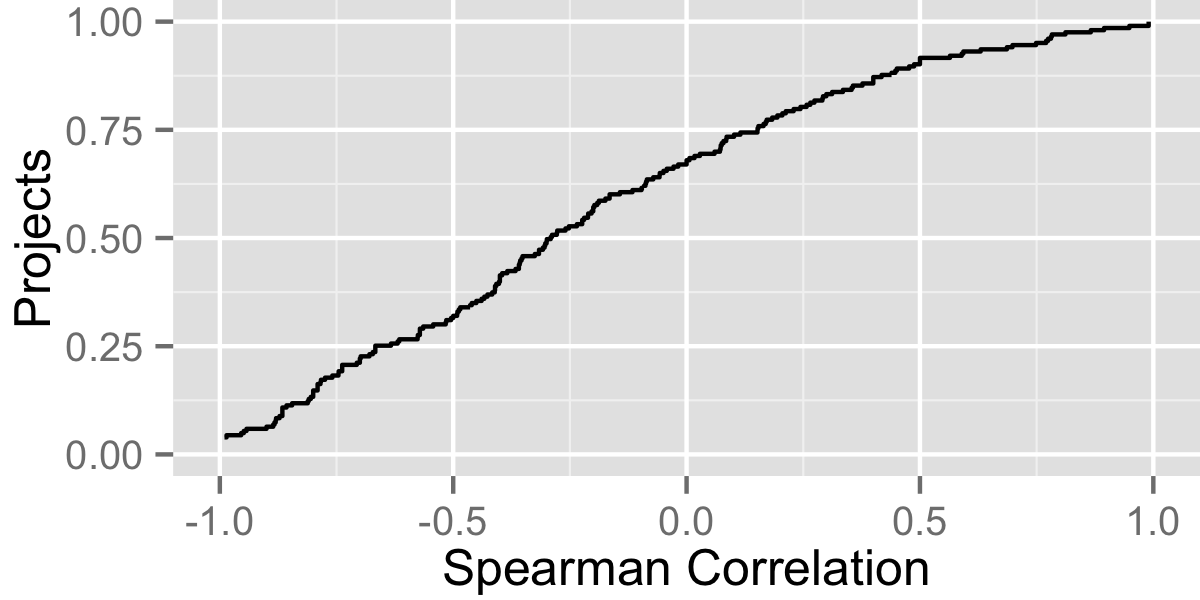
\includegraphics[width=0.45\textwidth]{../analysis/result/change_commits_distribution.png} 
\label{fig:change_spearman} 
\caption{Spearman ranking for the correlation between frequency of changes of files and the usage of types in mature projects}
\end{figure}
%
% DISCUSSION
%
\section{Discussion\label{discussion}}
% TODO: Tell the reader that this sections is speculative

In this section, we discuss the questions proposed in Section \ref{questions} based on the results above.
Section \ref{discussion-q1} shows that documentation is the main reason why Groovy developers use types, specially on the definition of their modules.
An analysis of local variables, private declarations and test classes in Section \ref{discussion-q2} supports the hypothesis that untyped declarations are used more frequently when readability or stability are not a concern
Section \ref{discussion-q3} discusses the higher usage of untyped declarations in most Groovy projects.
Finally, Section \ref{discussion-q4} shows how programmers with experience using statically typed languages use types more frequently than other programmers.



% Q1
\subsection{Types as implicit documentation\label{discussion-q1}}
Well documented code plays an important role in making code more readable, hence improving the code overall maintainability \cite{Iso2004}.
By analyzing the results presented in Section \ref{results}, we were able to find evidence that this is an important factor considered by Groovy programmers.


% The second paragraph of this section says that the only motivation
% developers may have for putting in types is documentation, because you are
% ignoring the annotation that causes the compiler to check types. But how
% do you know that the developer was ignoring it? How can you conclude
% something about the developers motivation while ignoring one of the
% possibilities?

It is well known that the main advantages of using statically typed languages are implicit code documentation, static type verification and execution performance \cite{type_systems,mayer2012static}.
Groovy however is not a statically typed language, but a dynamically typed language with optional typing (we are not considering the $@TypeChecked$ annotation in this study).
This means that Groovy compiler can not verify types statically and that types still have to be checked during execution, which degrades runtime performance.
Hence from the usual advantages of using a statically typed language, only code documentation holds true for Groovy.
Considering the result shown on previous section, which shows that 60\% of all declarations are typed, this means that code documentation is an important matter for Groovy developers.

It is possible to observe an even higher usage of typing in the definition of modules.
As stated in related literature \cite{Meyer88, Meijer04, Wadler04, Plosch97, Flanagan2006, Furr09}, types greatly aid in the definition of the contract of a module.
They restrict the pre and post conditions of methods and define the nature of the properties of that module.
Therefore, clients of a well typed module learn how to use the module faster and make less mistakes since the contract of that module is clear to them.

Declarations that define the interface of a module, i.e, fields, returns and parameters of methods and parameters of constructors, are more typed than the average.
Figure \ref{fig:tipo_declaracao} shows that, while most of these elements are typed, only 30\%  of the local variables, which do not contribute to the definition of a module, are typed. On the other hand, parameters of constructors, which are some of the most important elements of a contract definition, are almost always typed \cite{Meijer04}. 

The results presented above above are further refined by visibility in Figures \ref{fig:method_return_visibility}, \ref{fig:method_parameter_visibility}, \ref{fig:constructor_parameter_visibility} and \ref{fig:field_visibility}.
They show that types are indeed considered more often on the definition of modules.
First, notice that declarations of private fields or methods are always less typed than their public and protected counterparts.
Private declarations are similar to local variables since they do not contribute to the interface of a module and are only accessible to the module where they were defined.
In this case there is a smaller need for documentation and programmers do not feel as compelled to use types.

Public and protected elements define the interface of a method and thus tend to be typed often.
In the case of parameters and returns of methods, the usage of types in declarations with protected visibility  surpasses that of methods and fields with public visibility.
In Groovy, protected declarations restrict access to internal elements of a class to its subclasses or other classes in the same package.
It can be argued that the relationship between these classes is tightly coupled \cite{Chidamber94}.
Apparently programmers understand that this type of contract is more delicate than others and that it should be well document.

The usage of types in public declarations is heavily influenced by the project size.
Figure \ref{fig:size_pubMethodReturn} shows this clearly.
In projects with more than 65KLoC, these untyped declarations are seen with less than half the frequency observed in the smallest projects.
However, no particular pattern can be observed for private or protected declarations, presented in Figures \ref{fig:size_priMethodReturn} and \ref{fig:size_proMethodReturn}.

Intuitively, the larger the project, the greater the difficulty of integration and the need for maintenance.
This is more critical in public methods and fields.
Unlike private or protected declarations, the number of modules to which a public methods or field is visible grows with the project size.
This suggests that as projects grow, programmers realize that the documentation of public elements is more important and consider typing these declarations more often.

The project size has an opposite effect on the declarations of local variables.
While public declarations get typed more often, the frequency of types in local variable declarations decreases.
It is hard to tell the reason for this behavior.
A possible explanation is that, as project grows, developers get more used to flexibility and objectivity of dynamic typing.
They stop typing their declarations unless they understand they are really necessary.

% Q2
\subsection{Less typing when readability and stability are not a concern\label{discussion-q2}}
When readability or stability are not a concern, the advantages of typing become less apparent and  programmers seem to prefer the flexibility of untyped declarations.
This is what we found when we analyzed how typing is used in local variables, private declarations and test classes.
These are scenarios where we consider readability and stability to be less relevant.

Most local variables are untyped.
Figure \ref{fig:tipo_declaracao} shows that less than 30\% of these variables are declared with a type, a value significantly smaller than the overall result for all declaration types, 60\%.
It can be assumed that typing local variables does not aid in the readability of the code as much as in other types of declarations.
The value of a local variable is defined very close to its declaration, usually in the same statement.
This makes it easier for a reader to understand the nature of a given variable and even infer its type.
Programmers can be more objective in this scenario and eliminate the repetitive work of typing their variables.

Local variables have a smaller scope.
They are only visible inside the block where they were instantiated and are destroyed once the execution of that block is over.
Stability in this scenario is not as critical making the flexibility of untyped declarations more clear.
For example, one can easily change the type of a local variable without having to worry about its use anywhere else.

A similar conclusion can be derived for declarations of private methods, fields and constructors.
As shown in Figures \ref{fig:method_return_visibility}, \ref{fig:method_parameter_visibility}, \ref{fig:constructor_parameter_visibility} and \ref{fig:field_visibility}, untyped declarations are much more common in in these declarations that in their public or private counterparts.
Private elements are usually more stable than others.
Since they are only visible inside the class they were defined in, they can often be changed without having any unexpected effects outside that class.
Also, since those elements are only referenced inside the class where they were defined, a reader can easily find those references and use them as a means to understand the code.

Another scenario with smaller need for readability and stability are test classes.
These classes usually have simple relationships with the rest of the project, not having any clients and depending only on the classes under test.
Test code is frequently considered a peripheral artifact of a software project and programmers usually do not worry about maintaining the quality of such code \cite{Meszaros07}.

Test classes are also typed less often than the average.
Figure \ref{fig:test_classes} shows that declarations made inside the main classes of a project are typed in 68\% of the cases.
On the other hand, only 56\% of the test classes are typed.

% TODO If scripts are as throwaway as the text suggests, then why are they stored in Github?
A counter example to this analysis is the usage of types in scripts.
It can also be said that readability and stability are not big concerns in scripts.
These are pieces of code usually written to solve punctual problems.
They do not establish complex relationships with other modules and are not reused very often.
Nevertheless, as shown in Table \ref{fig:scripts}, there is no significant difference between the overall usage of types in scripts and classes.

% Q3
\subsection{Frequently changed files have more untyped declarations\label{discussion-q3}}
As stated in Question Q3, there are reasons to use typed and reasons to use untyped declarations in files that change often.
Types improve the readability of code by implicitly documenting statements \cite{should_your_specification_language_be_typed}.
On the other hand, it is easier to change untyped code \cite{gradual_typing}.
The results presented in Section \ref{res-changes} however show that the latter is considered more often than the first.

Figure \ref{fig:change_spearman} shows clearly that for most projects, the usage of untyped declarations grows as the frequency of changes in a file increases.
Apparently, programmers understand that untyped code makes maintenance tasks easier.
One can argue that the causal relationship is inverted, i.e., these files have to be changed more often because of problems generated by the use of untyped declarations.
However, it is very unlikely that programmers would not notice that untyped declarations would be causing such problems and would not add types to those declarations in order to fix them.

An important conclusion that can be extracted from this analysis is that types are not absolutely necessary in order to build a maintainable system.
At least, in most software projects written in Groovy, where there is a higher need for maintenance, programmers seem to prefer the flexibility of untyped declarations over the readability of types.


% Q4
\subsection{Programmers used to static typing use types more often\label{discussion-q4}}
Results indicate that the answer for Question Q4 is affirmative.
The choice for using types on a language with optional typing, such a Groovy, is in fact influenced by the experience  with other languages.
Those developers who have only static languages on their GitHub portfolio leave their declarations untyped less often than other developers.
Figure \ref{fig:untyped_background} shows that these developers have only 28.7\% of their declarations untyped compared to 40\% of those developers with dynamic languages on their portfolio. 











%
% THREATS TO VALIDITY
%
\section{Threats to Validity\label{threats}}
In this section, we discuss potential threats to validity. As usual, we have arranged possible threats in two categories, internal and external validity \cite{Wohlin2012}. 

\subsection*{Internal Validity}
The main threats to the internal validity involve the fact that, in such a large scale empirical study, we can not analyze data in much detail. 
In Section \ref{res-background} we consider that the GitHub portfolio of a programmer represents well his experience with other languages and type systems, but this might not be true for all programmers.
They may have projects in their portfolio that they have not worked on or projects hosted somewhere else written in other languages.
There is still the possibility of a programmer having multiple GitHub accounts with different languages in each one, causing this programmer to be counted twice with different inferred backgrounds.
Due to the large number of programmers considered in our study, we expect these special cases not to have a large influence over the results.

% TODO
I% n Section \ref{res-size}, we consider that the project size is a metric capable of representing the complexity of a project, but this is not always true \cite{Fenton1998}.
% However that was the most effective metric we could use without requiring projects to be compiled, which would drastically reduce the number of % projects in our dataset.

There are other factors which might have influenced programmers besides the ones considered in this study.
Some frameworks require programmers to use typed or untyped declarations in some cases.
For example, one of the ways a programmer can create a stub object in Spock, a popular Groovy testing framework, requires programmers to type the mock declaration.
In addition to that, the previous experience of programmers, which we have shown to have influence over programmers, might interfere with the analysis of other influencing factors.

In order to overcome the threats shown above, we are planning a controlled study as a future work.
This will provide us with more detailed information, which we can use to complement the results of this empirical study.

\subsection*{External Validity}
Although we have analyzed a very extensive number of Groovy projects, it can not be said that we have all possible scenarios covered.
By manually inspecting our dataset, we could find only a few projects with characteristics of software developed inside an organization.
Most of them were developed by small groups of people or open source communities.
It is probable that such enterprise projects are hosted privately on GitHub or in private servers, hence unavailable to us.

The behavior observed for Groovy projects can be very different in other languages.
Most languages are not like Groovy and feature either static or dynamic typing, forcing programmers to choose a single typing strategy for all scenarios in a single project.
Even a language with a hybrid typing paradigm might implement different strategies which will be perceived differently by the programmers of that language.

Finally, a programmer must consider other features in the choice for a programming language like tool support, available libraries and the preferences of his or her organization.
If these are the features considered in such choice, a programmer might end with the typing paradigm that is not ideal for his or her specific context.











%
% RELATED WORK
%
\section{Related Work\label{related}}
This work is based on a series of studies that compare different typing strategies.
Although we are not aware of any studies that analyze this question using a large scale case study as ours, we know of multiple controlled experiments with significant results.

In \cite{experiment_with_purity}, the author compares the performance of two groups of students asked to develop two small systems. 
Both groups used a language developed by the author, Purity. 
The only difference in the language used by the two groups was the type system.
One group used a statically typed version of Purity while the other used a dynamically typed version of the same language.
Results showed that the group using the dynamic version was significantly more productive than the other. 
Similarly to this work, the author was able to compare two typing strategies directly while isolating any external factors. 
However, it can be argued that these results may not represent well real life situations in the software industry. 
This was a short duration study where students were used as examples of developers with no interaction with other programmers. 
In our study, we try to get more relevant results when analyzing source code developed by programmers during their normal activities.

In a follow up study \cite{hanenberg_icpc}, the authors obtained opposite conclusions. 
They compared the performance of two groups of developers in maintenance tasks. 
The first group used Java, a statically typed language, and the other used Groovy, but restricting developers to use only untyped declarations in order to simulate a dynamically typed version of Java.
In this case, the group using the statically typed language, Java, was much more productive.
This contradiction with a previous work reinforces the argument that the results of controlled studies are not reliable enough for this type of study.

In experiments conducted in \cite{ruby_vs_druby}, the authors compare the performance of two groups working on small development tasks.
One group used Ruby, a dynamically typed language, while the other used DRuby, a statically typed version of Ruby. 
Results showed that the DRuby compiler rarely managed to capture any errors that were not already evident for programmers.
Most subjects involved in the study had previous experience with Ruby, which suggests that programmers get used to the lack of typing in their declarations.
We tried to investigate this phenomenon, by analyzing how programmers use types depending on their experience with other languages.











%
% CONCLUSION AND FUTURE WORK
%
\section{Conclusions and Future Work\label{conclusion}}
In this study, we investigated, from a practical point of view, what are the most influential factors on the choice of a programmer for using or not types.
Understanding these factors can help programmers choosing the most appropriate programming language for a given context.
This information can also be valuable for programming language designers who can base their design on real user data.
To answer this question, we conducted a large scale case study with almost 7000 software projects written in Groovy, a dynamically typed language with optional type annotations. 

We found evidence that programmers use types as a means to implicitly document their code.
This tends to grow in the presence of some factors, such as the visibility, the complexity of the contract defined by such declaration and the size of the project where it was defined. 
Conversely, when readability or stability are not a concern, the simplicity and flexibility of untyped declarations seems to be preferred, as seen on local variables, private declarations and test classes.
Another important factor is the previous experience of programmers with a given type system.

In future work we wish to analyze the influence of static and dynamic type systems over the robustness of software systems.
In particular, we want to understand whether the use of dynamic typing, which limits the compiler's ability to find type problems, has any correlation with the occurrence of defects in the system and if the use of automated testing is able to reduce this correlation.


\acks
This work was partially supported by FAPEMIG, grants APQ-02376-11 and APQ-02532-12.

\newpage 

%
% BIBLIOGRAPHY
%
\bibliographystyle{abbrvnat}
\renewcommand{\bibfont}{\normalsize}
\begin{thebibliography}{}
\softraggedright

\bibitem[Tiobe Website(2013)]{tiobe}
Tiobe programming community index. http://www.tiobe.com/index.php/ content/paperinfo/tpci/index.html. Accessed in 23/09/2013.

\bibitem[Groovy(2013)]{groovy}
Groovy Programming Language. http://groovy.codehaus.org/. Accessed in 10/10/2013.

\bibitem[Bruce, K. (2002)]{bruce2002foundations}
Bruce, K. (2002). Foundations of object-oriented languages: types and semantics. MIT press.

\bibitem[Bruch, M., Monperrus, M., and Mezini, M. (2009)]{bruch2009learning}
Bruch, M., Monperrus, M., and Mezini, M. (2009). Learning from examples to improve code completion systems. In Proceedings of the the 7th joint meeting of the European software engineering conference and the ACM SIGSOFT symposium on The foundati- ons of software engineering, pages 213–222. ACM.

\bibitem[Cardelli, L. (1996]{type_systems}
Cardelli, L. (1996). Type systems. ACM Comput. Surv., 28(1):263–264.

\bibitem[Chang, M., Mathiske, B., Smith, E., Chaudhuri, A., Gal, A., Bebenita, M., Wimmer, C.]{jit}
Chang, M., Mathiske, B., Smith, E., Chaudhuri, A., Gal, A., Bebenita, M., Wimmer, C., and Franz, M. (2011). The impact of optional type information on jit compilation of dynamically typed languages. SIGPLAN Not., 47(2):13–24.

\bibitem[Daly, M. T., Sazawal, V., and Foster, J. S. (2009)]{ruby_vs_druby}
Daly, M. T., Sazawal, V., and Foster, J. S. (2009). Work In Progress: an Empirical Study of Static Typing in Ruby. In Workshop on Evaluation and Usability of Programming Languages and Tools (PLATEAU), Orlando, Florida.

\bibitem[Hanenberg, S. (2010)]{experiment_with_purity}
Hanenberg, S. (2010). An experiment about static and dynamic type systems: doubts about the positive impact of static type systems on development time. SIGPLAN Not., 45(10):22–35.

\bibitem[Kleinschmager, S., Hanenberg, S., Robbes, R., and Stefik, A. (2012)]{hanenberg_icpc}
Kleinschmager, S., Hanenberg, S., Robbes, R., and Stefik, A. (2012). Do static type systems improve the maintainability of software systems? An empirical study. 2012 20th IEEE International Conference on Program Comprehension (ICPC), pages 153– 162.

\bibitem[Lamport, L. and Paulson, L. C. (1999)]{should_your_specification_language_be_typed}
Lamport, L. and Paulson, L. C. (1999). Should your specification language be typed. ACM Trans. Program. Lang. Syst., 21(3):502–526.

\bibitem[Mayer,C.,Hanenberg,S.,Robbes,R.,Tanter,E ́.,andStefik,A.(2012)]{mayer2012static}
Mayer,C.,Hanenberg,S.,Robbes,R.,Tanter,E ́.,andStefik,A.(2012). Static type systems (sometimes) have a positive impact on the usability of undocumented software: An empirical evaluation. self, 18:5.

\bibitem[Pierce, B. (2002)]{types_and_programming_languages}
Pierce, B. (2002). Types and programming languages. MIT press.

\bibitem[Tratt, L. (2009)]{dynamically_typed_languages}
Tratt, L. (2009). Chapter 5 dynamically typed languages. volume 77 of Advances in Computers, pages 149 – 184. Elsevier.

\bibitem[Siek, Jeremy, and Walid Taha(2007)]{gradual_typing}
Siek, Jeremy, and Walid Taha. "Gradual typing for objects." ECOOP 2007–Object-Oriented Programming. Springer Berlin Heidelberg, 2007. 2-27.

\bibitem[Gray(2008)]{gray08}
Gray, K. E. Safe cross-language inheritance. In European Conference on Object-Oriented Programming (2008), pp. 52–75.

\bibitem[Gray(2011)]{gray11}
Gray, K. E. Interoperability in a scripted world: Putting inheritance \& prototypes together. In Foundations of Object-Oriented Languages (2011).

\bibitem[Gray(2005)]{gray05}
Gray, K. E., Findler, R. B.,Andflatt, M. Fine-grained interoperability through contracts and mirrors. InObject-Oriented Programming, Systems, Languages, and Applications(2005), pp. 231–245.

\bibitem[Siek(2007)]{siek07}
Siek, J.,Andtaha, W. Gradual typing for objects. In European Conference on Object-Oriented Programming(2007),pp. 2–27.

\bibitem[Takikawa(2012)]{takikawa12}
Takikawa, Asumu, et al. "Gradual typing for first-class classes." ACM SIGPLAN Notices. Vol. 47. No. 10. ACM, 2012.
\bibitem[Fowler(2010)]{fowler10}
Fowler, Martin. Domain-specific languages. Pearson Education, 2010.

% Types help on the definition of a contract
\bibitem[Meijer(2004)]{Meijer04}
Meijer, Erik, and Peter Drayton. "Static typing where possible, dynamic typing when needed: The end of the cold war between programming languages." OOPSLA, 2004.

\bibitem[Wadler(2004)]{Wadler04}
Wadler, Philip, and Robert Bruce Findler. "Well-typed programs can’t be blamed." Programming Languages and Systems. Springer Berlin Heidelberg, 2009. 1-16.

% Unfortunately, dynamically typed programming languages usually do not support the concept of DEC. Therefore we integrated DEC into the programming language Python by using a metaprogramming approach
\bibitem[Plosch(1997)]{Plosch97}
Plosch, Reinhold. "Design by contract for Python." Software Engineering Conference, 1997. Asia Pacific and International Computer Science Conference 1997. APSEC'97 and ICSC'97. Proceedings. IEEE, 1997.

%Traditional static type systems are very effective for verifying basic interface specifications
\bibitem[Flanagan(2006)]{Flanagan2006}
Flanagan, Cormac. "Hybrid type checking." ACM Sigplan Notices. Vol. 41. No. 1. ACM, 2006.

\bibitem[Meyer(1988)]{Meyer88}
Meyer, Bertrand. Object-oriented software construction. Vol. 2. New York: Prentice hall, 1988.

\bibitem[Furr(2009)]{Furr09}
Furr, Michael, et al. "Static type inference for Ruby." Proceedings of the 2009 ACM symposium on Applied Computing. ACM, 2009.

\bibitem[Meszaros(2007)]{Meszaros07}
Meszaros, Gerard. xUnit test patterns: Refactoring test code. Pearson Education, 2007.

% Coupling is high for inheritance
% interaction coupling, component coupling and inheritance coupling
\bibitem[Chidamber(1994)]{Chidamber94}
Chidamber, Shyam R., and Chris F. Kemerer. "A metrics suite for object oriented design." Software Engineering, IEEE Transactions on 20.6 (1994): 476-493.

\bibitem[ISO25000(2004)]{Iso2004}
ISO, ISO, and IEC FCD. "25000, Software Engineering-Software Product Quality Requirements and Evaluation (SQuaRE)-Guide to SQuaRE." Geneva, International Organization for Standardization (2004).

\bibitem[Fenton(1998)]{Fenton1998}
Fenton, Norman E., and Shari Lawrence Pfleeger. Software metrics: a rigorous and practical approach. PWS Publishing Co., 1998.

\bibitem[Wohlin(2012)]{Wohlin2012}
Wohlin, Claes, et al. Experimentation in software engineering. Springer Publishing Company, Incorporated, 2012.

\end{thebibliography}


\end{document}

%                       Revision History
%                       -------- -------
%  Date         Person  Ver.    Change
%  ----         ------  ----    ------

%  2013.06.29   TU      0.1--4  comments on permission/copyright notices

